% Options for packages loaded elsewhere
\PassOptionsToPackage{unicode}{hyperref}
\PassOptionsToPackage{hyphens}{url}
%
\documentclass[
]{book}
\usepackage{amsmath,amssymb}
\usepackage{iftex}
\ifPDFTeX
  \usepackage[T1]{fontenc}
  \usepackage[utf8]{inputenc}
  \usepackage{textcomp} % provide euro and other symbols
\else % if luatex or xetex
  \usepackage{unicode-math} % this also loads fontspec
  \defaultfontfeatures{Scale=MatchLowercase}
  \defaultfontfeatures[\rmfamily]{Ligatures=TeX,Scale=1}
\fi
\usepackage{lmodern}
\ifPDFTeX\else
  % xetex/luatex font selection
\fi
% Use upquote if available, for straight quotes in verbatim environments
\IfFileExists{upquote.sty}{\usepackage{upquote}}{}
\IfFileExists{microtype.sty}{% use microtype if available
  \usepackage[]{microtype}
  \UseMicrotypeSet[protrusion]{basicmath} % disable protrusion for tt fonts
}{}
\makeatletter
\@ifundefined{KOMAClassName}{% if non-KOMA class
  \IfFileExists{parskip.sty}{%
    \usepackage{parskip}
  }{% else
    \setlength{\parindent}{0pt}
    \setlength{\parskip}{6pt plus 2pt minus 1pt}}
}{% if KOMA class
  \KOMAoptions{parskip=half}}
\makeatother
\usepackage{xcolor}
\usepackage{longtable,booktabs,array}
\usepackage{calc} % for calculating minipage widths
% Correct order of tables after \paragraph or \subparagraph
\usepackage{etoolbox}
\makeatletter
\patchcmd\longtable{\par}{\if@noskipsec\mbox{}\fi\par}{}{}
\makeatother
% Allow footnotes in longtable head/foot
\IfFileExists{footnotehyper.sty}{\usepackage{footnotehyper}}{\usepackage{footnote}}
\makesavenoteenv{longtable}
\usepackage{graphicx}
\makeatletter
\def\maxwidth{\ifdim\Gin@nat@width>\linewidth\linewidth\else\Gin@nat@width\fi}
\def\maxheight{\ifdim\Gin@nat@height>\textheight\textheight\else\Gin@nat@height\fi}
\makeatother
% Scale images if necessary, so that they will not overflow the page
% margins by default, and it is still possible to overwrite the defaults
% using explicit options in \includegraphics[width, height, ...]{}
\setkeys{Gin}{width=\maxwidth,height=\maxheight,keepaspectratio}
% Set default figure placement to htbp
\makeatletter
\def\fps@figure{htbp}
\makeatother
\usepackage{soul}
\setlength{\emergencystretch}{3em} % prevent overfull lines
\providecommand{\tightlist}{%
  \setlength{\itemsep}{0pt}\setlength{\parskip}{0pt}}
\setcounter{secnumdepth}{5}
\usepackage{booktabs}
\usepackage{amsthm}
\makeatletter
\def\thm@space@setup{%
  \thm@preskip=8pt plus 2pt minus 4pt
  \thm@postskip=\thm@preskip
}
\makeatother
\ifLuaTeX
  \usepackage{selnolig}  % disable illegal ligatures
\fi
\usepackage[]{natbib}
\bibliographystyle{apalike}
\IfFileExists{bookmark.sty}{\usepackage{bookmark}}{\usepackage{hyperref}}
\IfFileExists{xurl.sty}{\usepackage{xurl}}{} % add URL line breaks if available
\urlstyle{same}
\hypersetup{
  pdftitle={CNC Fly Food Dispenser},
  pdfauthor={Matt Wayland},
  hidelinks,
  pdfcreator={LaTeX via pandoc}}

\title{CNC Fly Food Dispenser}
\author{Matt Wayland}
\date{2024-01-19}

\begin{document}
\maketitle

{
\setcounter{tocdepth}{1}
\tableofcontents
}
\hypertarget{preface}{%
\chapter*{Preface}\label{preface}}
\addcontentsline{toc}{chapter}{Preface}

\begin{center}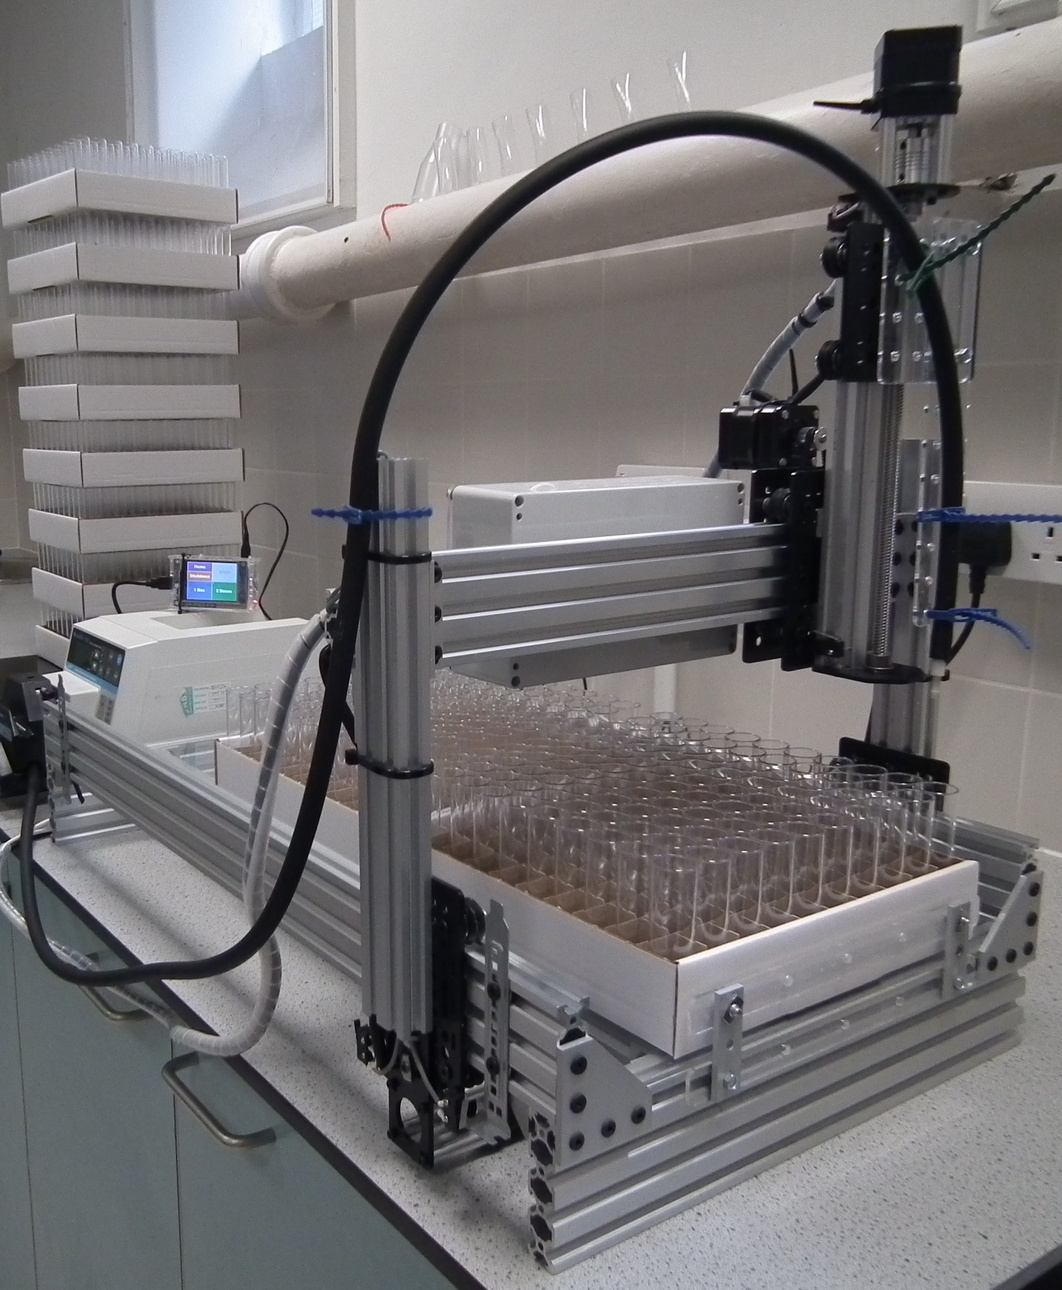
\includegraphics[width=0.75\linewidth]{images/system} \end{center}

\hypertarget{github}{%
\section*{Github}\label{github}}
\addcontentsline{toc}{section}{Github}

\href{https://github.com/WaylandM/fly-food-robot}{WaylandM/fly-food-robot}

\hypertarget{license}{%
\section*{License}\label{license}}
\addcontentsline{toc}{section}{License}

License for software and documentation:
\href{https://www.gnu.org/licenses/gpl-3.0.en.html}{GPL-3}

\hypertarget{contact}{%
\section*{Contact}\label{contact}}
\addcontentsline{toc}{section}{Contact}

Matt Wayland

\hypertarget{publication}{%
\section*{Publication}\label{publication}}
\addcontentsline{toc}{section}{Publication}

Article in \href{https://openhardware.metajnl.com/}{Journal of Open Hardware}:
\url{https://openhardware.metajnl.com/articles/10.5334/joh.9/}

\hypertarget{colophon}{%
\section*{Colophon}\label{colophon}}
\addcontentsline{toc}{section}{Colophon}

This book was produced using the \textbf{bookdown} package \citep{R-bookdown}, which was built on top of R Markdown and \textbf{knitr} \citep{xie2015}.

\hypertarget{intro}{%
\chapter{Introduction}\label{intro}}

The fruit fly, \emph{Drosophila melanogaster}, is one of the most important model organisms in biological research. Maintaining stocks of fruit flies in the laboratory is labour-intensive. One task which lends itself to automation is the production of the vials of food in which the flies are reared. Fly facilities typically have to generate several thousand vials of fly food each week to sustain their fly stocks. The system presented here combines a Cartesian coordinate robot with a peristaltic pump (Figure \ref{fig:architecture}). The design of the robot is based on the Routy CNC Router created by Mark Carew (\url{http://openbuilds.org/builds/routy-cnc-router-v-slot-belt-pinion.101/}), and uses belt and pully actuators for the X and Y axes, and a leadscrew actuator for the Z axis. CNC motion and operation of the peristaltic pump are controlled by grbl (\url{https://github.com/gnea/grbl}), an open source, embedded, high performance g-code parser. Grbl is written in optimized C and runs directly on an Arduino. A Raspberry Pi is used to generate and stream G-code instructions to Grbl. A touch screen on the Raspberry Pi provides a graphical user interface to the system. The system has capacity to fill two boxes of fly food vials at a time. Instructions for building the hardware are available on \href{http://docubricks.com/viewer.jsp?id=8652757760093769728}{DocuBricks}.

\begin{figure}

{\centering 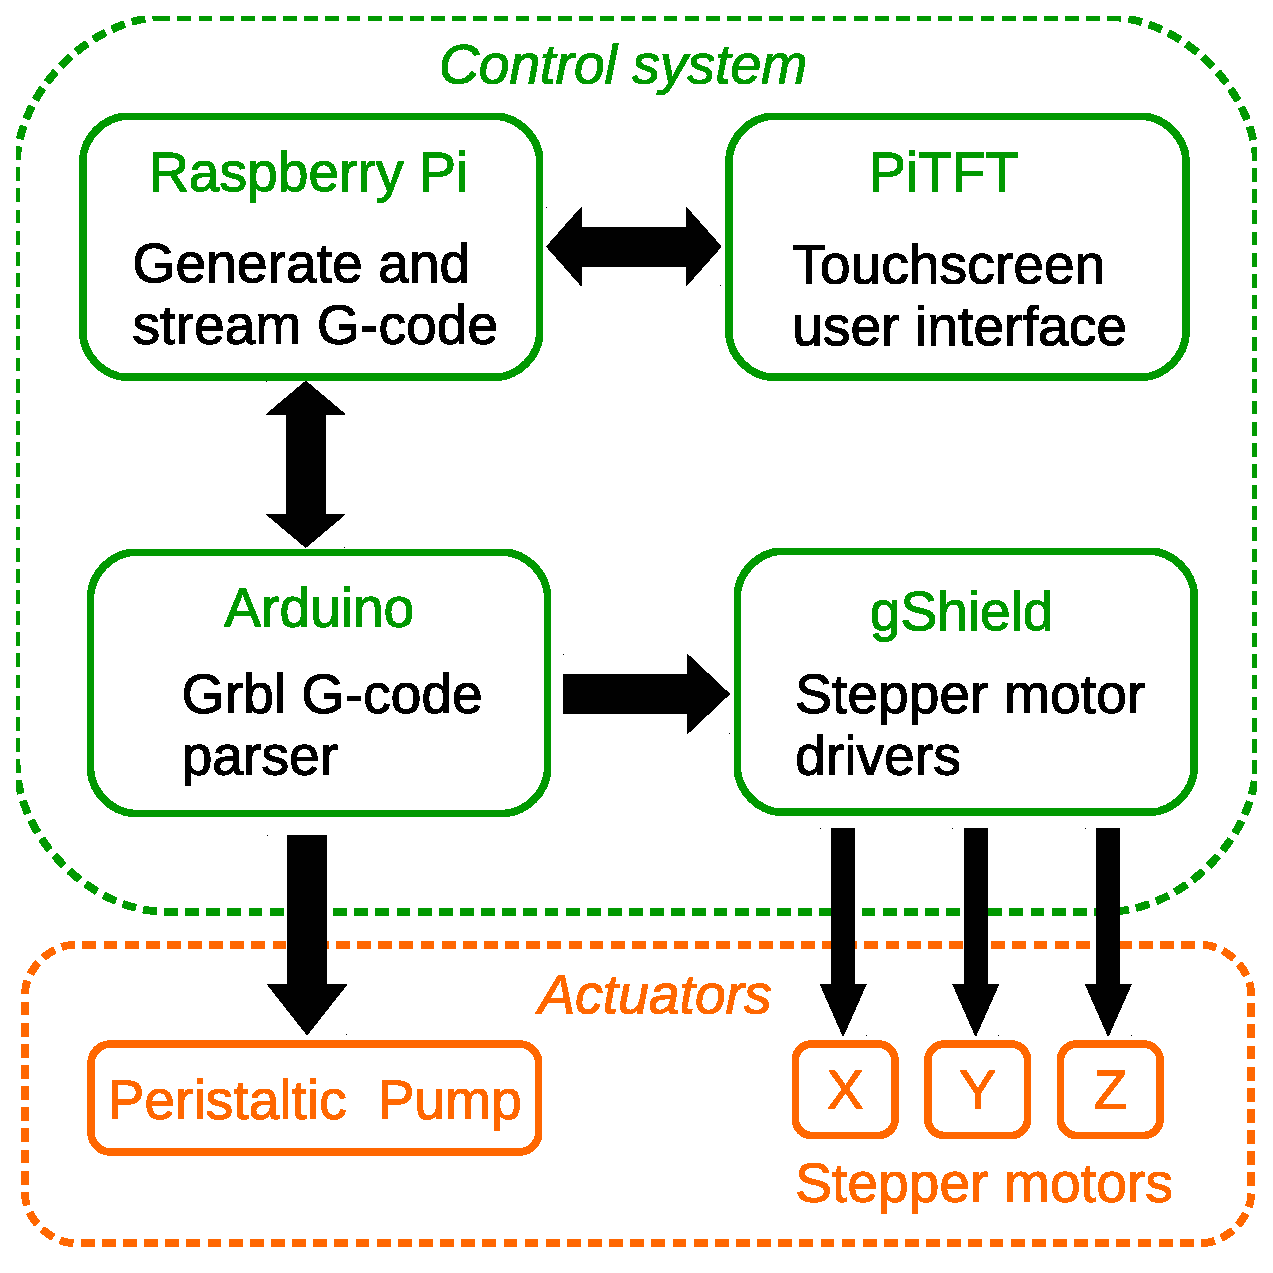
\includegraphics[width=0.75\linewidth]{images/system_architecture} 

}

\caption{System architecture.}\label{fig:architecture}
\end{figure}

Software installation and configuration on the Arduino and raspberry pi are detailed in chapters \ref{grbl} and \ref{raspi}. Chapter \ref{gcode} explains how to program the robot to fill vials of fly food. Instructions for the routine use of the robot are provided in chapter \ref{operation}. To see a video of the robot in action, go to:

\url{https://doi.org/10.6084/m9.figshare.5175223.v1}

An article providing an overview of this project has been published in the \href{https://openhardware.metajnl.com/}{Journal of Open Hardware}:
\url{https://openhardware.metajnl.com/articles/10.5334/joh.9/}

\hypertarget{grbl}{%
\chapter{Grbl installation and configuration}\label{grbl}}

\hypertarget{overview}{%
\section{Overview}\label{overview}}

CNC motion control is provided by grbl (\url{https://github.com/gnea/grbl}), an open source, embedded, high performance g-code parser. Grbl is written in optimized C and runs directly on an Arduino. This is used in conjunction with the gShield (formerly known as grblshield) which provides the hardware drivers for the stepper motors. Grbl sends out TTL signals on pins A3 and 13 of the Arduino to control coolant flow and spindle direction, respectively. Here these signals are used to remotely control a peristaltic pump.

\hypertarget{flashing-grbl-to-arduino}{%
\section{Flashing Grbl to Arduino}\label{flashing-grbl-to-arduino}}

To flash Grbl to the Arduino you will need a computer with the latest version of the \href{https://www.arduino.cc/en/Main/Software}{Arduino IDE} installed. The following instructions for flashing Grbl to the Arduino are taken from: \url{https://github.com/gnea/grbl/wiki/Compiling-Grbl}

\emph{\textbf{NOTE: Before starting, delete prior Grbl library installations from the Arduino IDE. Otherwise, you'll have compiling issues! On a Mac, Arduino libraries are located in \texttt{\textasciitilde{}/Documents/Arduino/libraries/}. On Windows, it's in \texttt{My\ Documents\textbackslash{}Arduino\textbackslash{}libraries}.}}

\begin{enumerate}
\def\labelenumi{\arabic{enumi}.}
\tightlist
\item
  Download the Grbl source code.
\end{enumerate}

\begin{itemize}
\tightlist
\item
  Open the following page in your web browser: \url{https://github.com/gnea/grbl}
\item
  Click on the \texttt{\textless{}\textgreater{}Code} Tab
\item
  Click the \texttt{Clone\ or\ Download} green button on the Grbl home page.
\item
  Click the \texttt{Download\ ZIP}
\item
  Unzip the download and you'll have a folder called \texttt{grbl-XXX}, where \texttt{XXX} is the release version.
\end{itemize}

\begin{enumerate}
\def\labelenumi{\arabic{enumi}.}
\setcounter{enumi}{1}
\tightlist
\item
  Launch the Arduino IDE (figure \ref{fig:arduinoIDE})
\end{enumerate}

\begin{itemize}
\tightlist
\item
  Make sure you are using the most recent version of the Arduino IDE!
\end{itemize}

\begin{figure}

{\centering 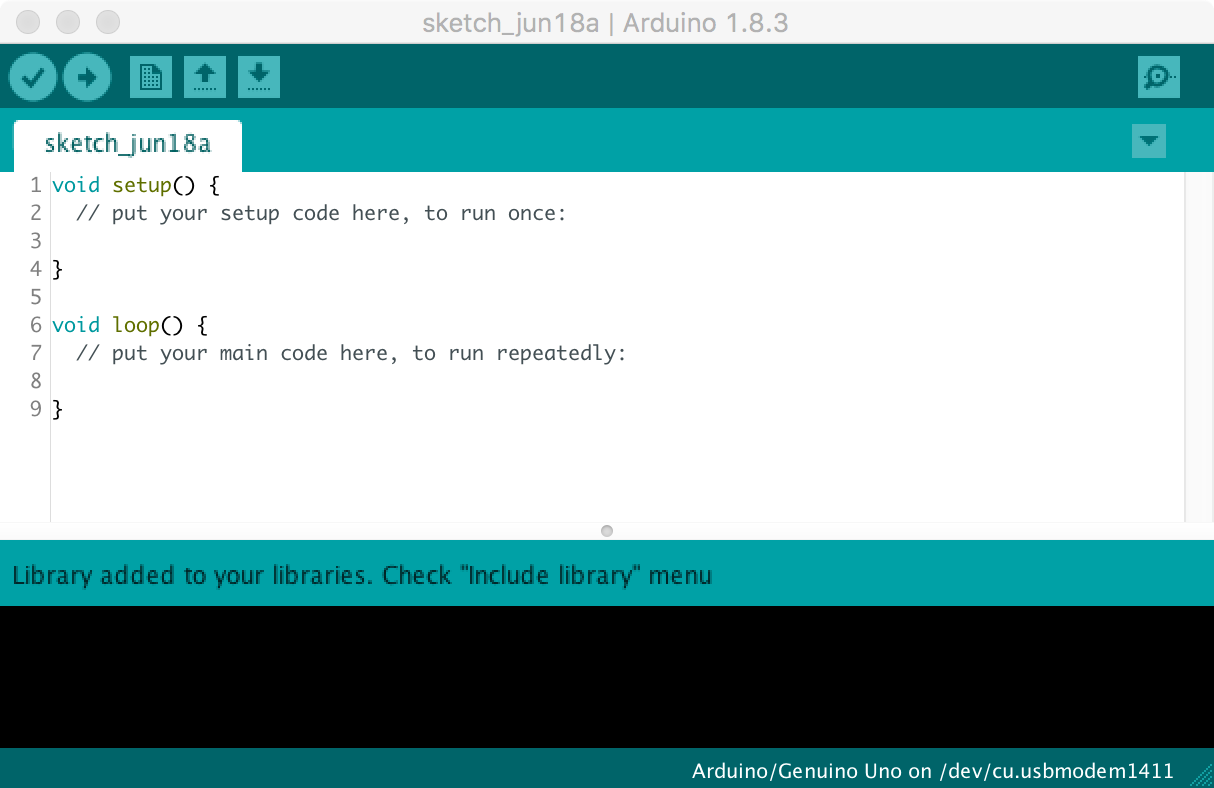
\includegraphics[width=0.75\linewidth]{images/arduino_IDE} 

}

\caption{Arduino IDE}\label{fig:arduinoIDE}
\end{figure}

\begin{enumerate}
\def\labelenumi{\arabic{enumi}.}
\setcounter{enumi}{2}
\tightlist
\item
  Load Grbl into the Arduino IDE as a Library.
\end{enumerate}

\begin{itemize}
\tightlist
\item
  Click the \texttt{Sketch} drop-down menu, navigate to \texttt{Include\ Library} and select \texttt{Add\ .ZIP\ Library}.
\item
  \textbf{IMPORTANT:} Select the \texttt{Grbl} folder \textbf{\emph{inside}} the \texttt{grbl-XXX} folder, which \textbf{only} contains the source files and an example directory (figure \ref{fig:addGrblLib}).
\end{itemize}

\begin{figure}

{\centering 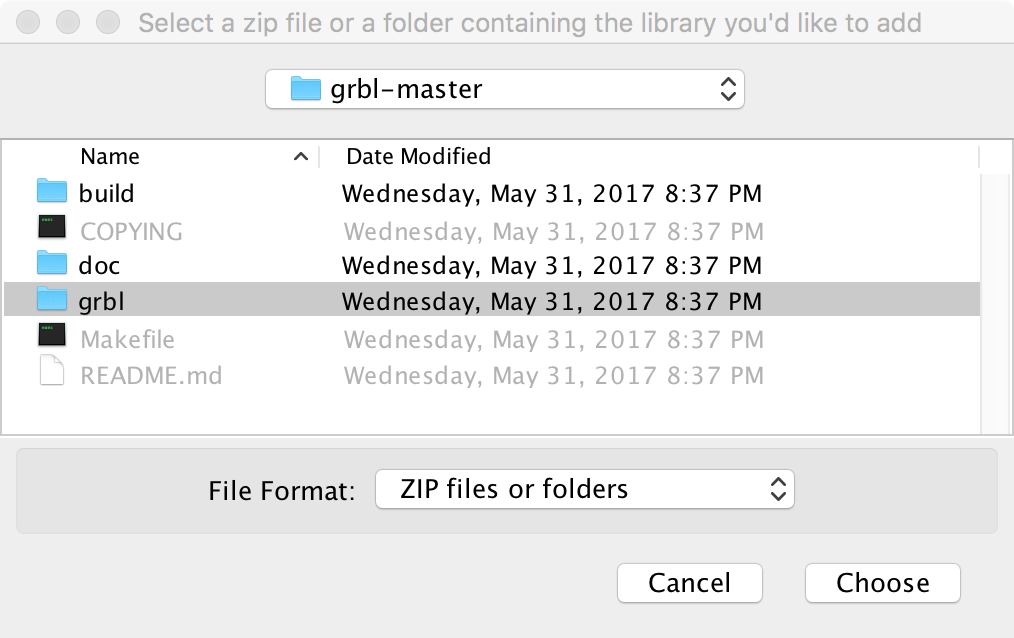
\includegraphics[width=0.75\linewidth]{images/add_grbl_lib} 

}

\caption{Loading Grbl library into the Arduino IDE}\label{fig:addGrblLib}
\end{figure}

\begin{itemize}
\tightlist
\item
  If you accidentally select the \texttt{.zip} file or the wrong folder, you will need to navigate to your Arduino library, delete the mistake, and re-do Step 3.
\end{itemize}

\begin{enumerate}
\def\labelenumi{\arabic{enumi}.}
\setcounter{enumi}{3}
\tightlist
\item
  Open the \texttt{GrblUpload} Arduino example.
\end{enumerate}

\begin{itemize}
\tightlist
\item
  Click the \texttt{File} drop-down menu, navigate to \texttt{Examples-\textgreater{}Grbl}, and select \texttt{GrblUpload} (figure \ref{fig:grblUploadFile}).
\end{itemize}

\begin{figure}

{\centering 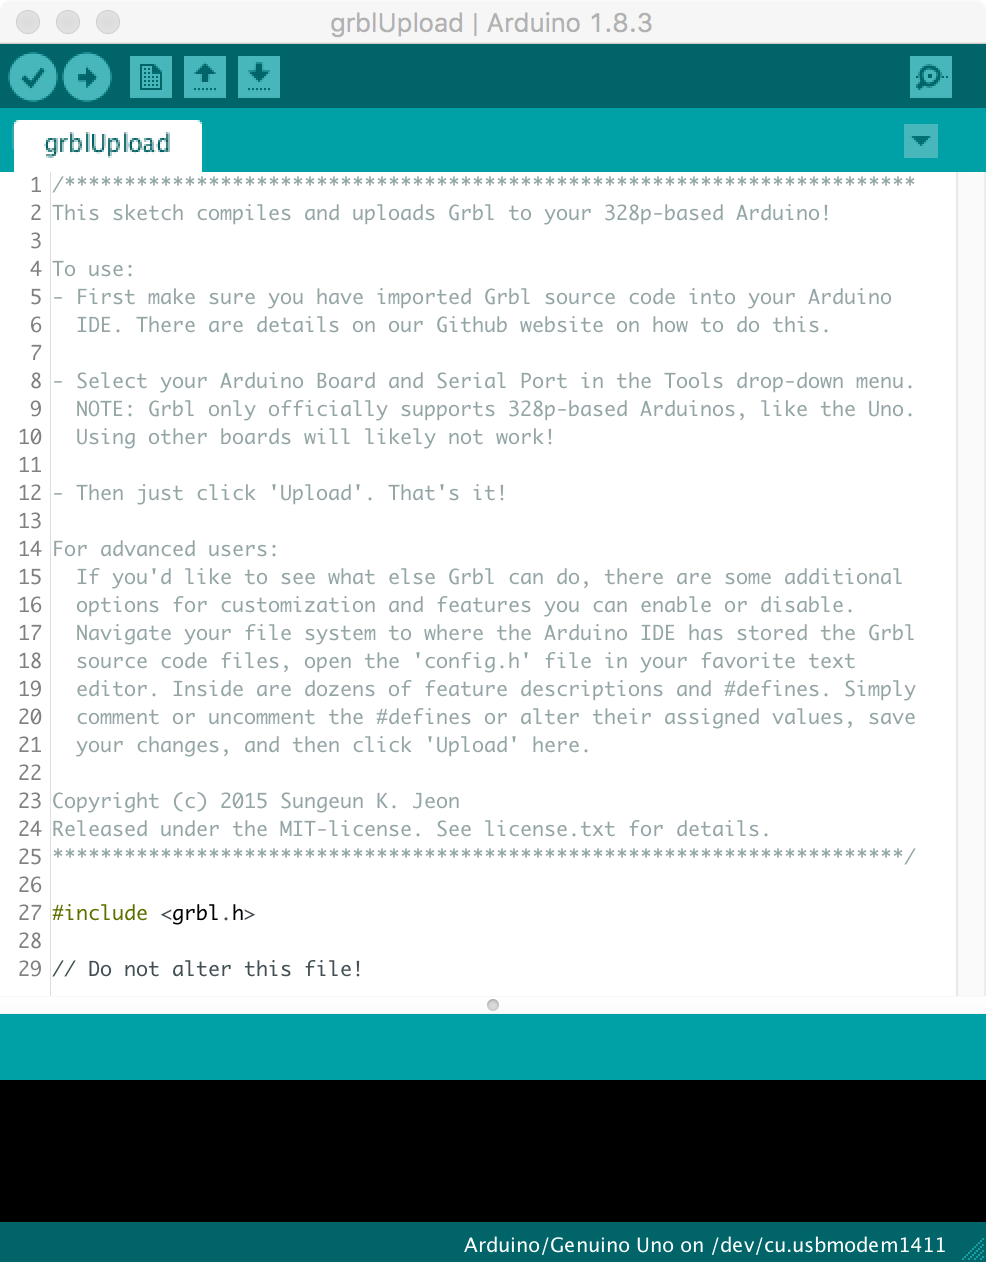
\includegraphics[width=0.75\linewidth]{images/grbl_upload_file} 

}

\caption{GrblUpload example file}\label{fig:grblUploadFile}
\end{figure}

\begin{enumerate}
\def\labelenumi{\arabic{enumi}.}
\setcounter{enumi}{4}
\tightlist
\item
  Compile and upload Grbl to your Arduino.
\end{enumerate}

\begin{itemize}
\tightlist
\item
  Connect your computer directly to the Arduino using the USB cable. Unplug the USB cable from the raspberry pi and plug it into your computer. Remember to reconnect the raspberry pi to the Arduino after you have finished configuring Grbl (figure \ref{fig:laptop2arduino}).
\end{itemize}

\begin{figure}

{\centering 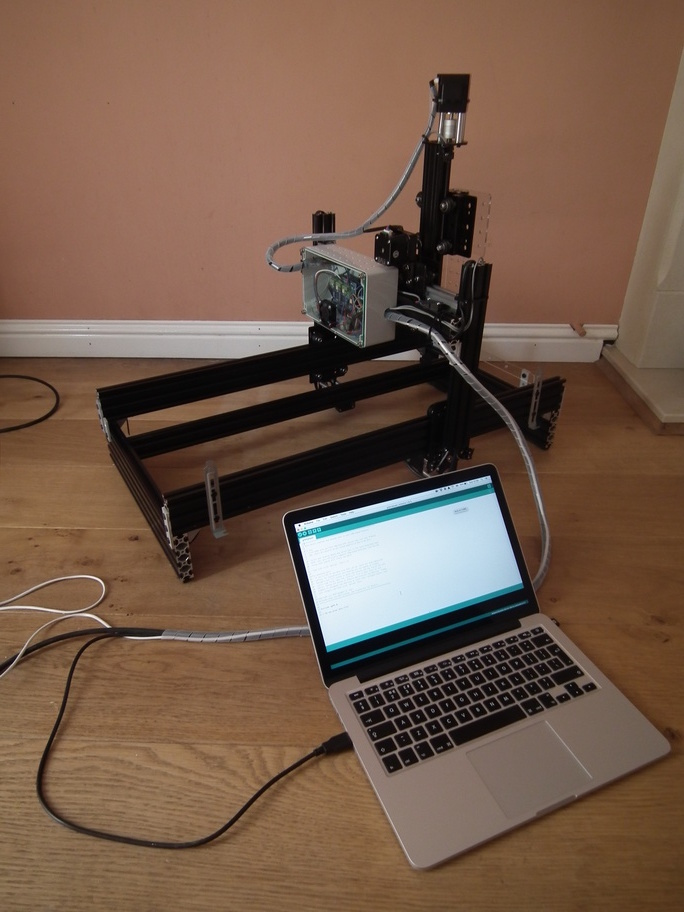
\includegraphics[width=0.75\linewidth]{images/laptop_connected_to_arduino} 

}

\caption{Laptop connected directly to Arduino}\label{fig:laptop2arduino}
\end{figure}

\begin{itemize}
\tightlist
\item
  Make sure your board is set to the Arduino Uno in the \texttt{Tool-\textgreater{}Board} menu and the serial port is selected correctly in \texttt{Tool-\textgreater{}Serial\ Port}.
\item
  Click the \texttt{Upload}, and Grbl should compile and flash to your Arduino! (Flashing with a programmer also works by using the \texttt{Upload\ Using\ Programmer} menu command.)
\end{itemize}

\hypertarget{check-serial-connection-to-grbl}{%
\section{Check serial connection to Grbl}\label{check-serial-connection-to-grbl}}

\emph{\textbf{NOTE: Before powering up the gShield and motors, check that the actuator carriages for all three axes are approximately centred (figure \ref{fig:actuatorsCentred}). Initially we do not know in which direction the actuator carriages will travel when G-code commands are issued, so positioning each in the middle of its range reduces the risk of collisions with the end stops.}}

\begin{figure}

{\centering 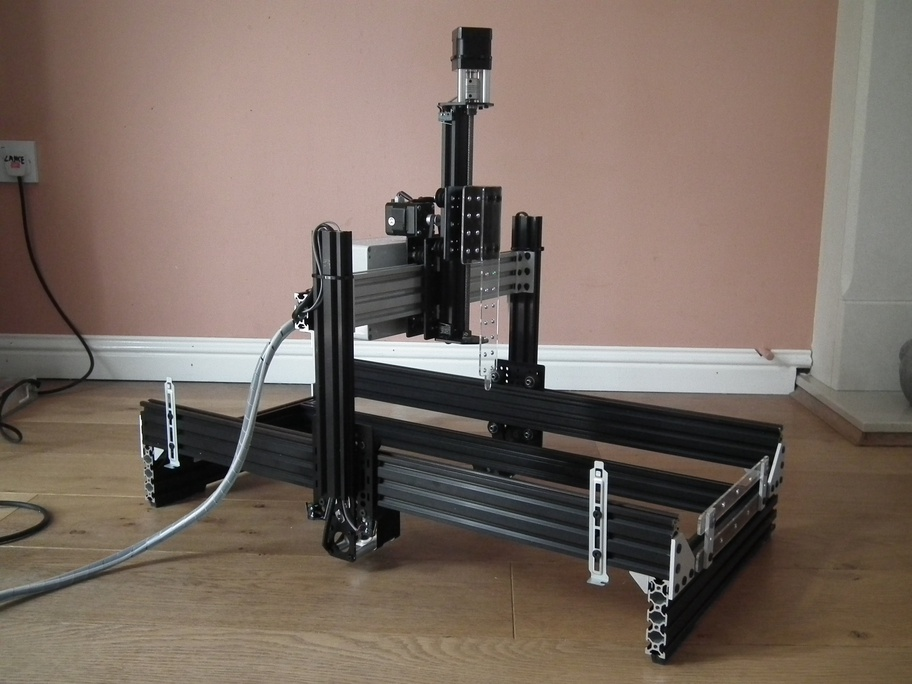
\includegraphics[width=0.75\linewidth]{images/actuator_carriages_centred} 

}

\caption{Actuator carriages centred in preparation for powering-up motors for first time}\label{fig:actuatorsCentred}
\end{figure}

\begin{enumerate}
\def\labelenumi{\arabic{enumi}.}
\tightlist
\item
  Open serial monitor in Arduino IDE
\end{enumerate}

\begin{itemize}
\tightlist
\item
  Click \texttt{Tools} drop-down menu, and select \texttt{Serial\ Monitor}
\end{itemize}

\begin{figure}

{\centering \includegraphics[width=0.75\linewidth]{images/Arduino_IDE_serial_monitor} 

}

\caption{Arduino IDE Serial Monitor}\label{fig:serialMonitor}
\end{figure}

\begin{itemize}
\tightlist
\item
  Note that line-ending is set to \texttt{Carriage\ return} and baud rate is set to \texttt{115200} (figure \ref{fig:serialMonitor})
\end{itemize}

\begin{enumerate}
\def\labelenumi{\arabic{enumi}.}
\setcounter{enumi}{1}
\tightlist
\item
  Try issuing a G-code command.
\end{enumerate}

\begin{itemize}
\tightlist
\item
  Type \texttt{?} and hit return.
\item
  This command will report the current position; as we have just started the system up all axes will be at 0.000.
\end{itemize}

\begin{enumerate}
\def\labelenumi{\arabic{enumi}.}
\setcounter{enumi}{2}
\tightlist
\item
  Now try moving actuators
\end{enumerate}

\begin{itemize}
\tightlist
\item
  To move in the x-axis type \texttt{x5} and hit return. Make a note of the direction in which the actuator carriage moves. N.B. this command tells Grbl to move to the x coordinate that is 5 units from the origin, it is not equivalent to telling the robot to move 5 units in the x-axis.
\item
  To move in the opposite direction along the x-axis type \texttt{x-5} and hit return.
\item
  To return to the starting point, use \texttt{x0}
\item
  Repeat for the other axes, replacing the x in the commands with y or z. Make a note of the direction the actuator carriages move with each command.
\end{itemize}

\hypertarget{grbl-configuration}{%
\section{Grbl configuration}\label{grbl-configuration}}

\hypertarget{read-current-configuration}{%
\subsection{Read current configuration}\label{read-current-configuration}}

\begin{itemize}
\tightlist
\item
  The \texttt{\$\$} command will report Grbl's current configuration.
\item
  Descriptions of these settings can be found here: \url{https://github.com/gnea/grbl/wiki/Grbl-v1.1-Configuration}
\item
  These settings will be modified in subsequent steps.
\end{itemize}

\hypertarget{check-directionality-of-each-axis.}{%
\subsection{Check directionality of each axis.}\label{check-directionality-of-each-axis.}}

\begin{figure}

{\centering 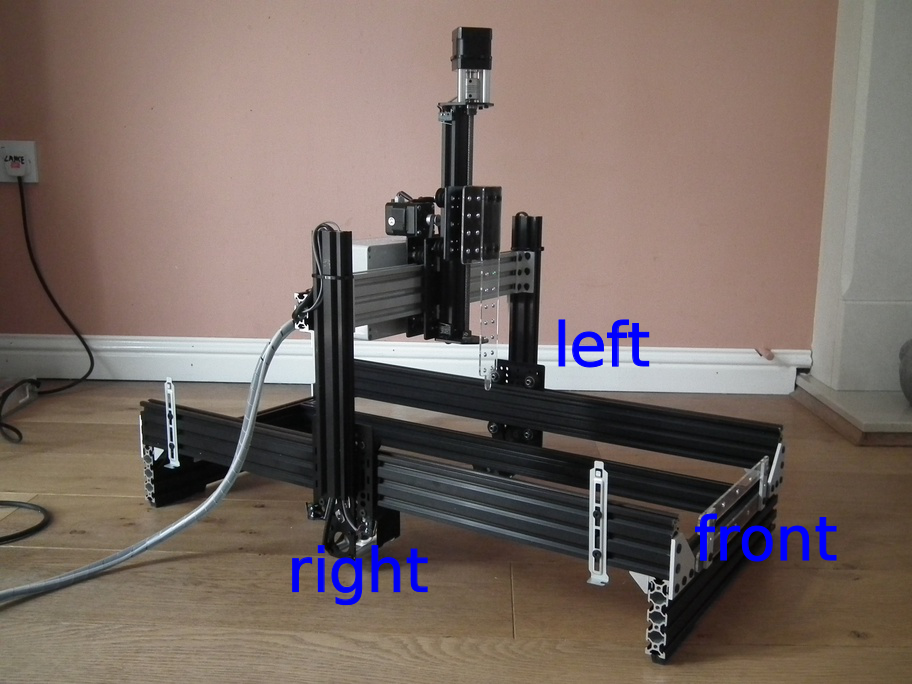
\includegraphics[width=0.75\linewidth]{images/robot_orientation} 

}

\caption{Orientation of robot.}\label{fig:robotOrientation}
\end{figure}

\begin{itemize}
\tightlist
\item
  Orientation of the robot is shown in figure \ref{fig:robotOrientation}.
\item
  At present the origins of all three axes are mid-way along each actuator, because this was the position of the actuator carriages when the system was started.
\item
  Make sure actuator carriages are at their current origin by entering this command: \texttt{x0y0z0}
\item
  Enter the command: \texttt{x5}. The x-axis carriage should move from right to left (orientation of robot is shown in figure \ref{fig:robotOrientation}. If it doesn't, make a note that it will need to be inverted.
\item
  Enter the command: \texttt{y5}. The y-axis carriage should move forwards. If it doesn't, make a note that it will need to be inverted.
\item
  Enter the command: \texttt{z5}. The z-axis carriage should move up. If it doesn't, make a note that it will need to be inverted.
\item
  The direction of the actuators can be inverted using setting \textbf{\$3}, the \href{https://github.com/gnea/grbl/wiki/Grbl-v1.1-Configuration\#3--direction-port-invert-mask}{Direction port invert (mask)}. An appropriate value is selected from table \ref{tab:invertMaskSettings}. For example, to invert the direction of the X and Z axis actuators use the following command: \texttt{\$3=5}
\end{itemize}

\begin{table}

\caption{\label{tab:invertMaskSettings}Masks for direction port inversion.}
\centering
\begin{tabular}[t]{lllll}
\toprule
Setting Value & Mask & Invert X & Invert Y & Invert Z\\
\midrule
0 & 00000000 & N & N & N\\
1 & 00000001 & Y & N & N\\
2 & 00000010 & N & Y & N\\
3 & 00000011 & Y & Y & N\\
4 & 00000100 & N & N & Y\\
\addlinespace
5 & 00000101 & Y & N & Y\\
6 & 00000110 & N & Y & Y\\
7 & 00000111 & Y & Y & Y\\
\bottomrule
\end{tabular}
\end{table}

\hypertarget{activate-hard-limits}{%
\subsection{Activate hard limits}\label{activate-hard-limits}}

Hard limits are a safety feature to prevent the machine from travelling beyond the limits of travel. Grbl monitors the paired limit switches on each axis and if a switch is triggered it will immediately switch off all motors. Hard limits are activated by setting \textbf{\$21} \href{https://github.com/gnea/grbl/wiki/Grbl-v1.1-Configuration\#21---hard-limits-boolean}{hard limits ( boolean)} to 1:

\begin{verbatim}
$21=1
\end{verbatim}

\hypertarget{setup-homing}{%
\subsection{Setup homing}\label{setup-homing}}

The homing cycle is used to set the origin of the Cartesian coordinate system used by the robot. During the homing cycle Grbl moves each actuator in the positive direction until the limit switches are triggered. The homing cycle is activated by setting \textbf{\$22} \href{https://github.com/gnea/grbl/wiki/Grbl-v1.1-Configuration\#22---homing-cycle-boolean}{homing cycle (boolean)} to 1:

\begin{verbatim}
$22=1
\end{verbatim}

Initiate a homing cycle using the following command: \texttt{\$h}. All actuator carriages should move to the origin of their axes. The origin of the Cartesian coordinate system (home) for the robot is shown in figures \ref{fig:xyOrigin} and \ref{fig:zOrigin}

\begin{figure}

{\centering 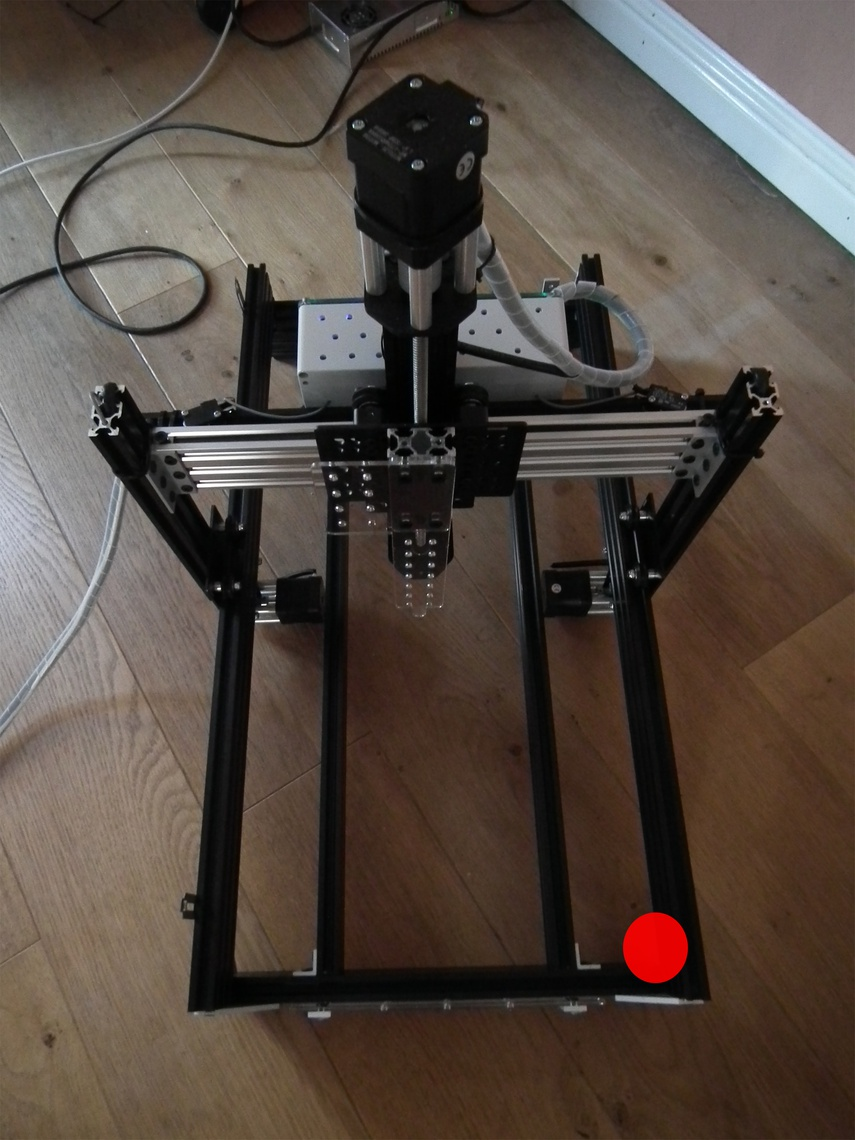
\includegraphics[width=0.75\linewidth]{images/xy_origin} 

}

\caption{Origin of XY coordinate system.}\label{fig:xyOrigin}
\end{figure}

\begin{figure}

{\centering 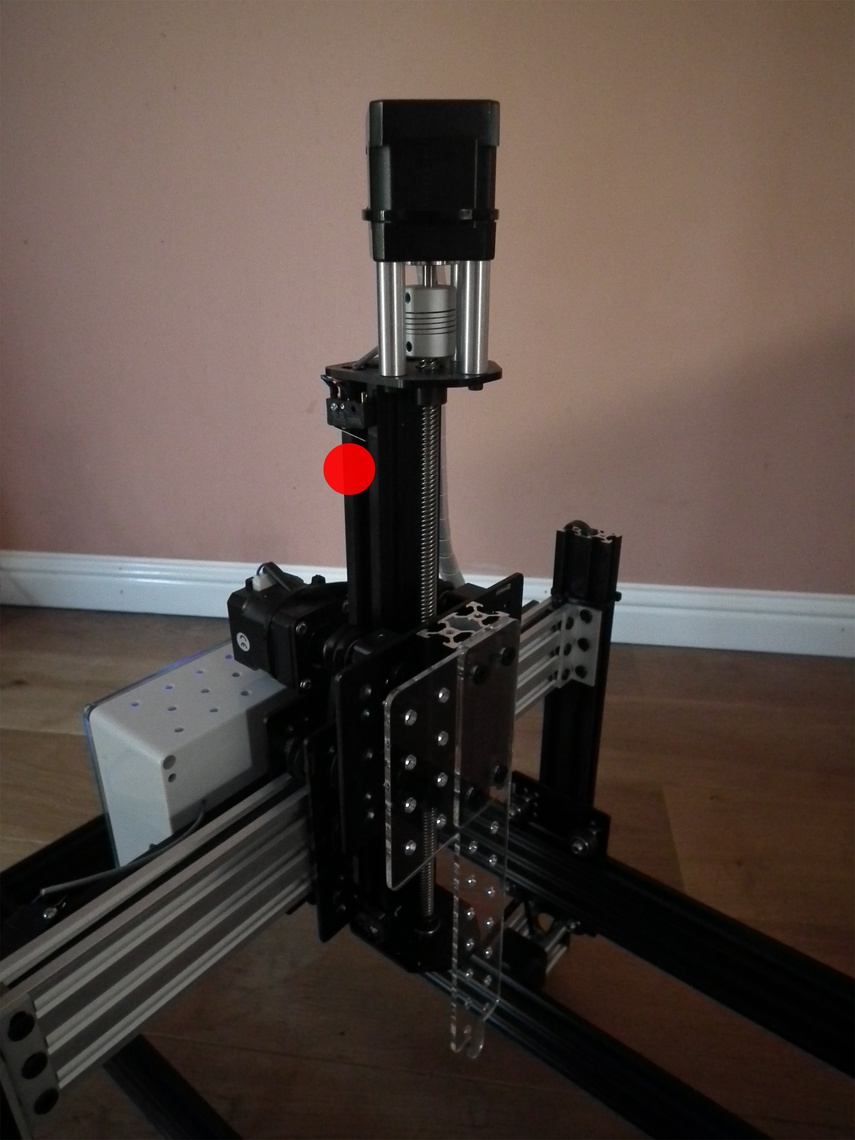
\includegraphics[width=0.75\linewidth]{images/z_origin} 

}

\caption{Origin of Z axis.}\label{fig:zOrigin}
\end{figure}

We also need to set \textbf{\$24} \href{https://github.com/gnea/grbl/wiki/Grbl-v1.1-Configuration\#24---homing-feed-mmmin}{homing feed rate} and \textbf{\$25} \href{https://github.com/gnea/grbl/wiki/Grbl-v1.1-Configuration\#25---homing-seek-mmmin}{homing seek rate}. Homing seek rate is the initial speed at which Grbl searches for the limit switches. Once it has them, it makes slower approach at the homing feed rate to get a more precise location for machine zero. We will set homing seek rate to 1000 mm/min \texttt{\$24=100} and homing feed rate to 100 mm/min \texttt{\$25=1000}.

At the end of a homing cycle each actuator carriage must be moved off its home limit switch, otherwise the hard limit will be triggered.
The \textbf{\$27} \href{https://github.com/gnea/grbl/wiki/Grbl-v1.1-Configuration\#27---homing-pull-off-mm}{Homing pull-off (mm)} specifies the distance required to clear the limit switches. For our robot we will use a value of 5mm:

\begin{verbatim}
$27=5
\end{verbatim}

\hypertarget{motor-step-size}{%
\subsection{Motor step size}\label{motor-step-size}}

\textbf{\$100}, \textbf{\$101} and \textbf{\$102} define \href{https://github.com/gnea/grbl/wiki/Grbl-v1.1-Configuration\#100-101-and-102--xyz-stepsmm}{{[}X,Y,Z{]} steps/mm}.
Suitable values for our stepper motors are:

\begin{verbatim}
$100=40
$101=40
$102=49.673
\end{verbatim}

If you are using a different type of stepper motor, the step size can be easily calculated by measuring how far each actuator moves in response to a G-code command. For example, we would calculate the step size for the X actuator as follows.

\begin{enumerate}
\def\labelenumi{\arabic{enumi}.}
\tightlist
\item
  Using the serial monitor in the Arduino IDE, issue the following command to \emph{home} the machine:
\end{enumerate}

\begin{verbatim}
$h
\end{verbatim}

\begin{enumerate}
\def\labelenumi{\arabic{enumi}.}
\setcounter{enumi}{1}
\tightlist
\item
  Read the current position of the machine, as reported by the Grbl controller:
\end{enumerate}

\begin{verbatim}
?
\end{verbatim}

After homing the Cartesian coordinates should be zero minus the homing pull-off:
* x = -5
* y = -5
* z = -5

\begin{enumerate}
\def\labelenumi{\arabic{enumi}.}
\setcounter{enumi}{2}
\item
  Make a note of the physical position of the nozzle.
\item
  Issue a g-code command to move to the -100mm position on the x-axis:
\end{enumerate}

\begin{verbatim}
x-100
\end{verbatim}

Keep decreasing the value of x until the x-actuator carriage almost meets the limit switch on the right hand side of the machine. The greater the distance moved, the more precise our calculation of step-size will be.

\begin{enumerate}
\def\labelenumi{\arabic{enumi}.}
\setcounter{enumi}{4}
\tightlist
\item
  Query Grbl's machine coordinates:
\end{enumerate}

\begin{verbatim}
?
\end{verbatim}

\begin{enumerate}
\def\labelenumi{\arabic{enumi}.}
\setcounter{enumi}{5}
\item
  Measure the physical distance travelled along the x-axis in millimetres.
\item
  Find \textbf{\$100}, the currently configured step size for the x-axis:
\end{enumerate}

\begin{verbatim}
$$
\end{verbatim}

\begin{enumerate}
\def\labelenumi{\arabic{enumi}.}
\setcounter{enumi}{7}
\tightlist
\item
  Calculate the correct value for step-size:
\end{enumerate}

\begin{verbatim}
current_step_size = steps/mm in current configuration
grbl_start = start position reported by Grbl controller (mm)
grbl_end = end position reported by Grbl controller (mm)
physical_distance = physical distance moved by actuator (mm)

steps/mm = -(curr_steps_per_mm * (end_pos_grbl-start_pos_grbl)) / physical_distance
\end{verbatim}

\hypertarget{feed-rates-and-acceleration}{%
\subsection{Feed rates and acceleration}\label{feed-rates-and-acceleration}}

\textbf{\$110}, \textbf{\$111} and \textbf{\$112} set the \href{https://github.com/gnea/grbl/wiki/Grbl-v1.1-Configuration\#110-111-and-112--xyz-max-rate-mmmin}{maximum rates (mm/min)} for the X, Y and Z actuators, respectively. We will use the following values:

\begin{verbatim}
$110=5000
$111=5000
$112=2500
\end{verbatim}

\href{https://github.com/gnea/grbl/wiki/Grbl-v1.1-Configuration\#120-121-122--xyz-acceleration-mmsec2}{Acceleration (mm/sec\^{}2)} is set to 50 for all axes:

\begin{verbatim}
$120=50
$121=50
$122=50
\end{verbatim}

\hypertarget{summary-of-settings}{%
\subsection{Summary of settings}\label{summary-of-settings}}

\begin{verbatim}
$0=10
$1=25
$2=0
$3=5
$4=0
$5=0
$6=0
$10=1
$11=0.010
$12=0.002
$13=0
$20=0
$21=1
$22=1
$23=0
$24=100.000
$25=1000.000
$26=250
$27=5.000
$30=1000
$31=0
$32=0
$100=40.000
$101=40.000
$102=49.673
$110=5000.000
$111=5000.000
$112=2500.000
$120=50.000
$121=50.000
$122=50.000
$130=200.000
$131=500.000
$132=200.000
\end{verbatim}

\hypertarget{setting-motor-current}{%
\section{Setting motor current}\label{setting-motor-current}}

The gShield has trimpots for adjusting the motor current of each axis, as shown in figure \ref{fig:gShield}.

\begin{figure}

{\centering 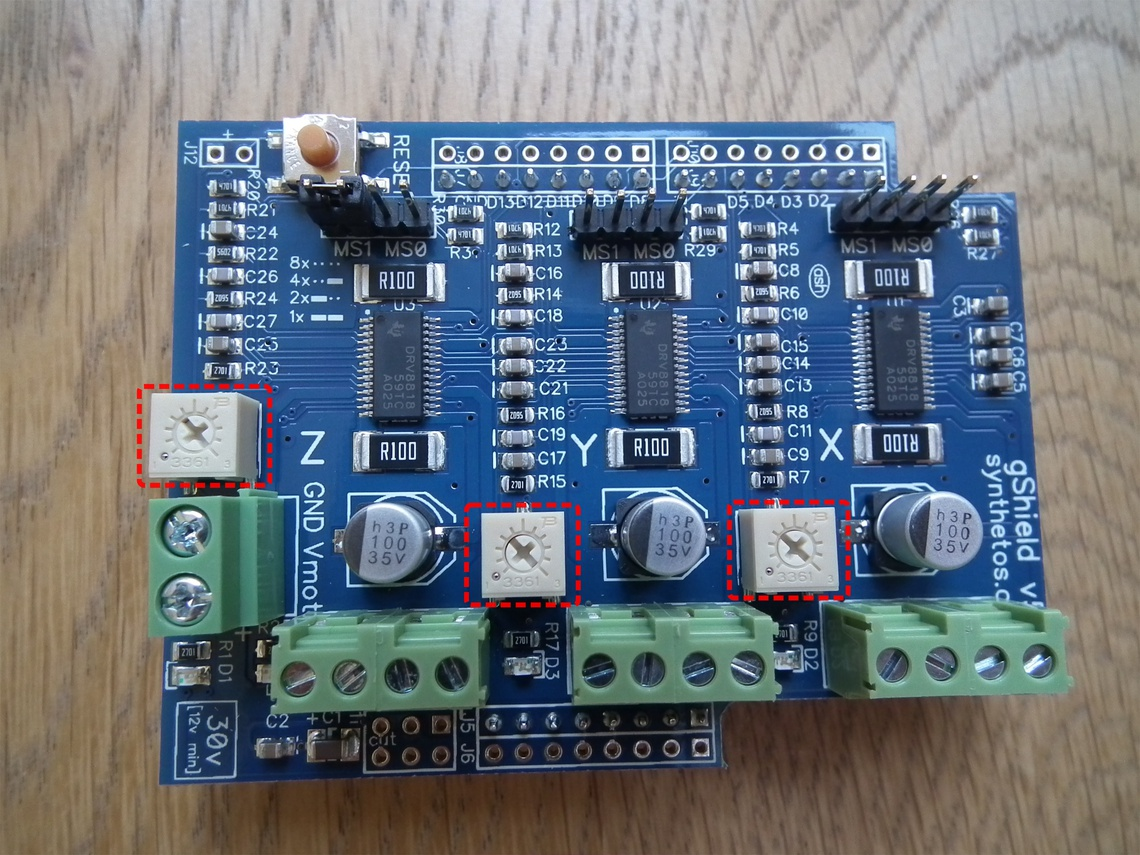
\includegraphics[width=0.75\linewidth]{images/gShield-trimpots} 

}

\caption{gShield trimpots}\label{fig:gShield}
\end{figure}

Instructions for setting motor current are provided here:
\url{https://github.com/synthetos/grblShield/wiki/Using-grblShield\#setting-motor-current}

\hypertarget{raspi}{%
\chapter{Raspberry Pi setup}\label{raspi}}

\hypertarget{overview-1}{%
\section{Overview}\label{overview-1}}

The raspberry pi is used to generate, then stream g-code to the Arduino. A small thin-film-transistor (TFT) touchscreen serves as the user interface to the raspberry pi.

\hypertarget{install-image}{%
\section{Install image}\label{install-image}}

\st{The first step is to install Adafruit's custom raspberry pi image on the micro SD card. The custom image is described here:}

\st{\mbox{\texttt{https://learn.adafruit.com/adafruit-pitft-28-inch-resistive-touchscreen-display-raspberry-pi/easy-install}}}

\st{We want the classic version which boots into X by default, rather then the lite version that boots to the command line. The classic version can be downloaded from this link:}

\st{\mbox{\texttt{https://s3.amazonaws.com/adafruit-raspberry-pi/2016-10-18-pitft-28r.zip}}}

Adafruit's custom raspberry pi image is no longer available. I have created an image (pitft.img) based on Adafruit's original that is preconfigured for use with the robot. It can be downloaded from:

\url{https://zenodo.org/records/10534021}

Instructions on installing images on SD cards can be found here:

\url{https://www.raspberrypi.org/documentation/installation/installing-images/}

\hypertarget{network-configuration}{%
\section{Network configuration}\label{network-configuration}}

The small screen of the pitft makes using most applications quite tricky. Therefore the first thing we should do after installing the image is configure networking, so that we can access the raspberry pi remotely using ssh.

To set a static IP address for the ethernet adapter, edit the following lines of \texttt{/etc/dhcpcd.conf}:

\begin{verbatim}
interface eth0

static ip_address=192.168.1.3/24
static routers=192.168.1.254
static domain_name_servers=192.168.1.254
\end{verbatim}

\textbf{ip\_address}, \textbf{routers} and \textbf{domain\_name\_servers} should be set to values appropriate for your network.

To raspberry pi can then be accessed using ssh, \emph{e.g.}:

\begin{verbatim}
  ssh pi@192.168.1.3
\end{verbatim}

The default password for the \textbf{pi} user account is \textbf{raspberry}

\hypertarget{install-minicom}{%
\section{Install minicom}\label{install-minicom}}

\emph{N.B. Minicom is pre-installed on my pitft.img}

Minicom is useful for manual control of the robot and for editing grbl settings.

To install minicom run these two commands:

\begin{verbatim}
sudo apt-get update
sudo apt-get install minicom
\end{verbatim}

Before we can use minicom we need to enable serial:

\begin{verbatim}
sudo nano /boot/config.txt
\end{verbatim}

Change the last line of this file from

\begin{verbatim}
enable_uart=0
\end{verbatim}

to

\begin{verbatim}
enable_uart=1
\end{verbatim}

If you have not already done so, reconnect the raspberry pi to the arduino using the USB cable. To use minicom to connect to the grbl controller running on the arduino, use:

\begin{verbatim}
sudo minicom -D /dev/ttyACM0 -b115200
\end{verbatim}

\hypertarget{expand-filesystem}{%
\section{Expand filesystem}\label{expand-filesystem}}

Expand filesystem on micro SD card:

\begin{verbatim}
    sudo raspi-config
    (expand filesystem)
    sudo reboot
\end{verbatim}

\hypertarget{installScripts}{%
\section{Install python scripts}\label{installScripts}}

\emph{N.B. The python scripts are pre-installed on my pitft.img}

Make sure you are in pi's home directory:

\begin{verbatim}
cd
\end{verbatim}

Download and unpack robot.tar.gz

\begin{verbatim}
curl -O https://raw.githubusercontent.com/WaylandM/fly-food-robot/master/raspberrypi/robot.tar.gz
tar xzvf robot.tar.gz
\end{verbatim}

The \textbf{robot} directory contains two subdirectories: \textbf{nc} (g-code scripts) and \textbf{py} (python scripts).

To automatically launch the robot GUI when the raspberry pi starts up, we need to edit the autostart file for the pi user:

\begin{verbatim}
sudo nano /home/pi/.config/lxsession/LXDE-pi/autostart
\end{verbatim}

Add the following line to autostart:

\begin{verbatim}
@/home/pi/robot/py/fly_gui.py
\end{verbatim}

\hypertarget{startup}{%
\chapter{System start-up}\label{startup}}

\hypertarget{attach-norprene-tubing}{%
\section{Attach Norprene tubing}\label{attach-norprene-tubing}}

\begin{enumerate}
\def\labelenumi{\arabic{enumi}.}
\tightlist
\item
  Attach the nozzle end of the Norprene tubing to the holder on the Z-axis actuator using releasable cable ties (figure \ref{fig:attachNozzle}).
\end{enumerate}

\begin{figure}

{\centering 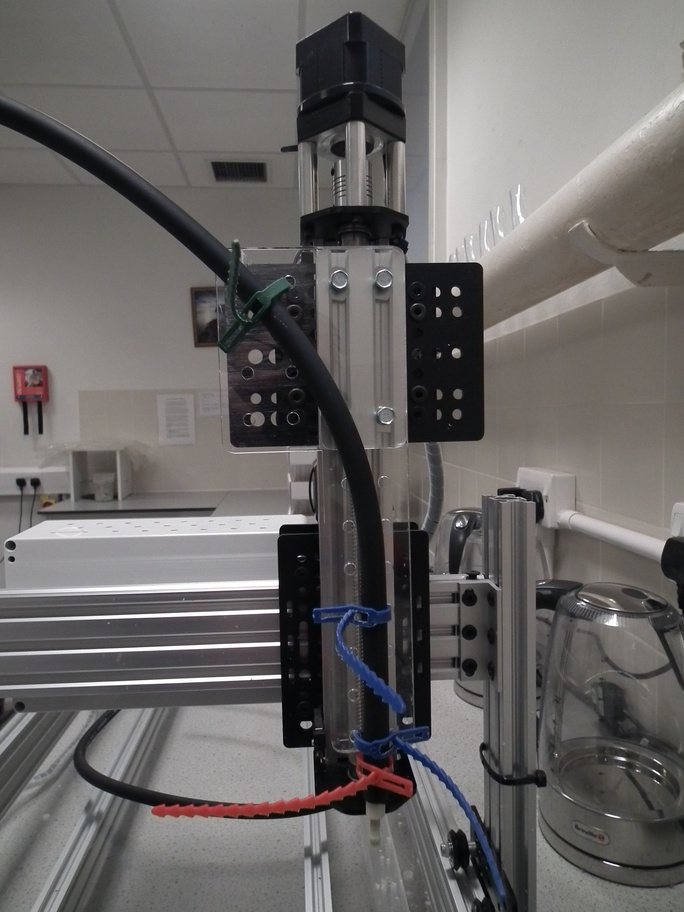
\includegraphics[width=0.75\linewidth]{images/pump4} 

}

\caption{Attachment of nozzle end of tubing to the Z-axis actuator.}\label{fig:attachNozzle}
\end{figure}

\begin{enumerate}
\def\labelenumi{\arabic{enumi}.}
\setcounter{enumi}{1}
\tightlist
\item
  Attach the Masterflex Norprene tubing to the right-hand side vertical post using a releasable cable tie. Ensure there is a large loop in the tubing between this attachment point and the nozzle so that the x-axis actuator can move freely (figure \ref{fig:tubingPost})
\end{enumerate}

\begin{figure}

{\centering 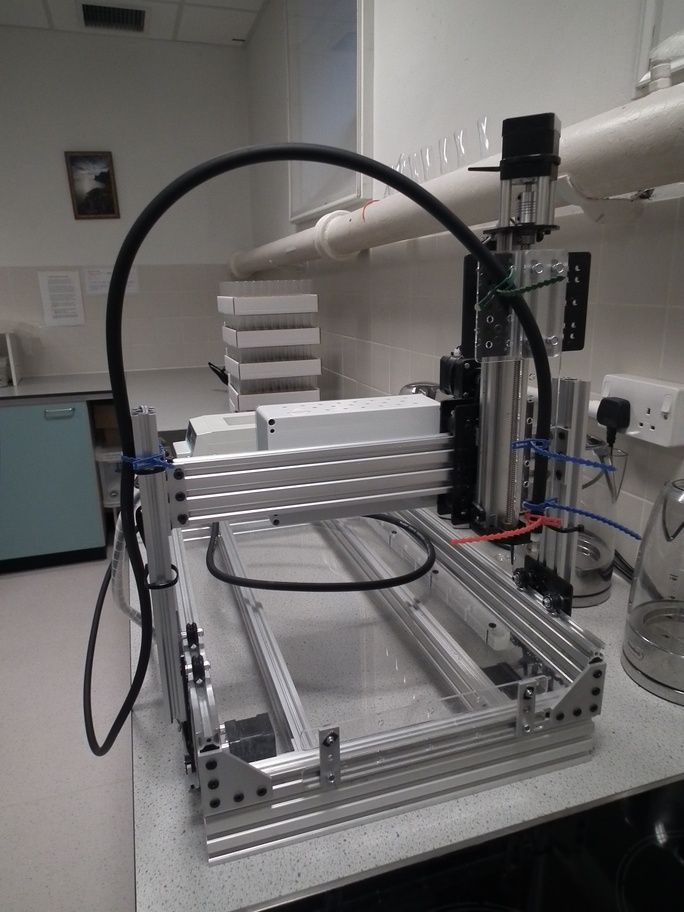
\includegraphics[width=0.75\linewidth]{images/pump5} 

}

\caption{Attachment of Norprene tubing to the right-hand side vertical post.}\label{fig:tubingPost}
\end{figure}

\begin{enumerate}
\def\labelenumi{\arabic{enumi}.}
\setcounter{enumi}{2}
\tightlist
\item
  Feed the tubing through the peristaltic pump (figure \ref{fig:tubingPump}) and into your vat of fly food (figure \ref{fig:flyFoodVat}).
\end{enumerate}

\begin{figure}

{\centering 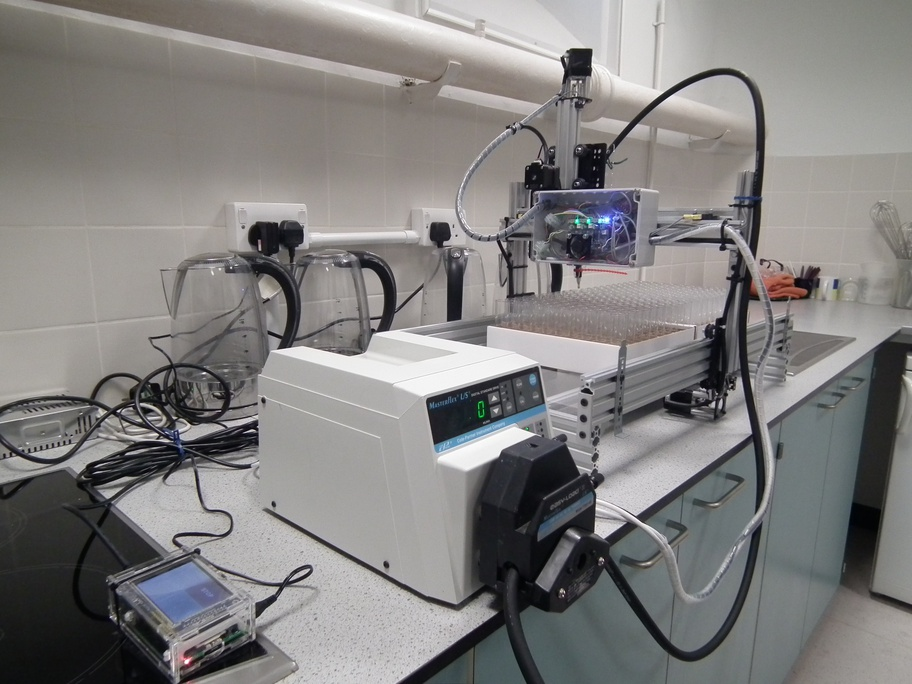
\includegraphics[width=0.75\linewidth]{images/pump6} 

}

\caption{Norprene tubing passing through peristaltic pump.}\label{fig:tubingPump}
\end{figure}

\begin{figure}

{\centering 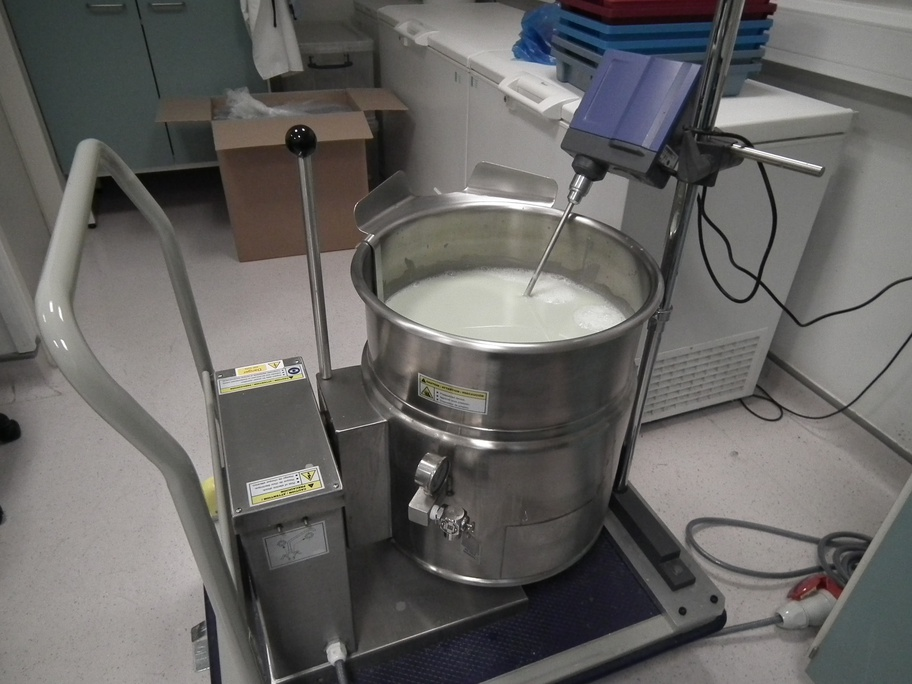
\includegraphics[width=0.75\linewidth]{images/pump7} 

}

\caption{Vat of fly food.}\label{fig:flyFoodVat}
\end{figure}

\hypertarget{switch-on-all-devices}{%
\section{Switch on all devices}\label{switch-on-all-devices}}

\begin{itemize}
\tightlist
\item
  power supply unit for gShield and motors
\item
  raspberry pi
\item
  peristaltic pump
\end{itemize}

\hypertarget{prime-pump}{%
\section{Prime pump}\label{prime-pump}}

\begin{itemize}
\tightlist
\item
  Position a beaker under the nozzle (figure \ref{fig:primeBeaker}).
\item
  Press and hold the prime button on the front of the peristaltic pump until a continuous stream of fly food is pumped into the beaker (figure \ref{fig:primeButton})
\end{itemize}

\begin{figure}

{\centering 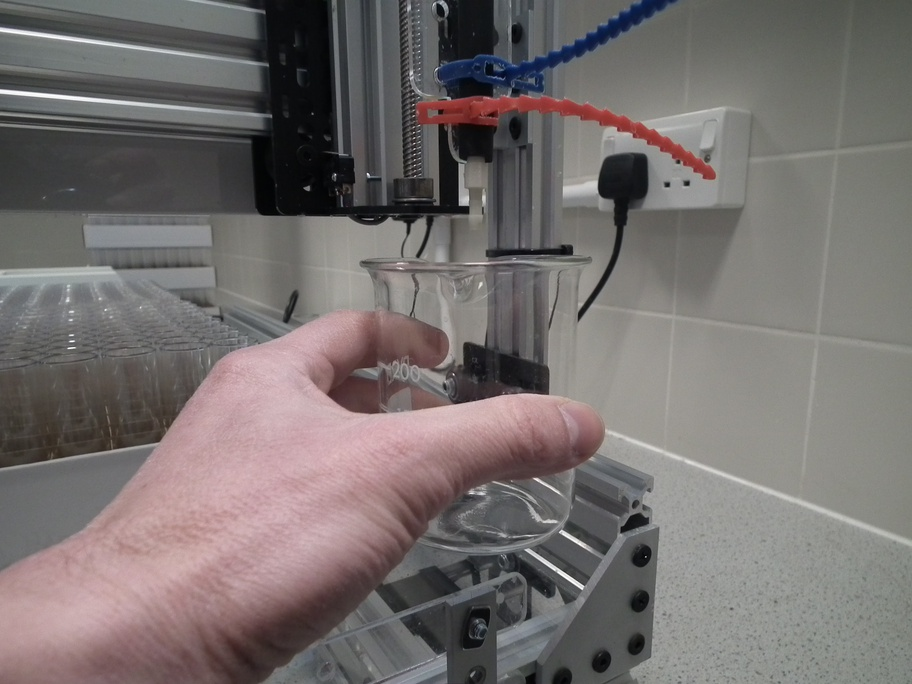
\includegraphics[width=0.75\linewidth]{images/prime_beaker} 

}

\caption{Positioning of beaker under nozzle to collect fly food expelled during priming of peristaltic pump.}\label{fig:primeBeaker}
\end{figure}

\begin{figure}

{\centering 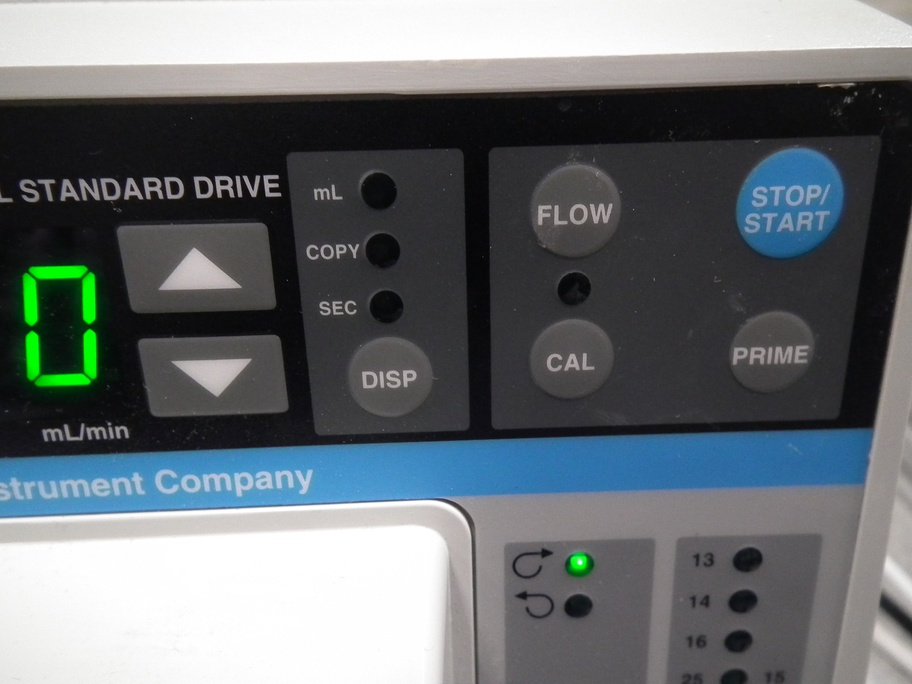
\includegraphics[width=0.75\linewidth]{images/prime_button} 

}

\caption{Prime button on peristaltic pump.}\label{fig:primeButton}
\end{figure}

\hypertarget{gcode}{%
\chapter{Program robot to fill vials}\label{gcode}}

\hypertarget{overview-2}{%
\section{Overview}\label{overview-2}}

The movement of the robot is programmed in \href{https://en.wikipedia.org/wiki/G-code}{G-code}. We only need nine G-code commands to control the robot (table \ref{tab:gCodes}).

\begin{table}

\caption{\label{tab:gCodes}G-code commands used to control robot.}
\centering
\begin{tabular}[t]{ll}
\toprule
Code & Description\\
\midrule
x & absolute position of x-axis\\
y & absolute position of y-axis\\
z & absolute position of z-axis\\
g4 & dwell time (control parameter p specifies seconds)\\
m3 & set pump rotation to clockwise\\
\addlinespace
m4 & set pump rotation to counter clockwise\\
m8 & start pump\\
m9 & stop pump\\
\$h & initiate homing cycle\\
\bottomrule
\end{tabular}
\end{table}

A G-code program for filling vials of food could be created manually, by listing the necessary commands sequentially in a text file. However, this would be laborious and error prone. If the size of the boxes of vials are known, the G-code can be programmatically generated.

\hypertarget{loadBoxes}{%
\section{Load boxes}\label{loadBoxes}}

\begin{figure}

{\centering 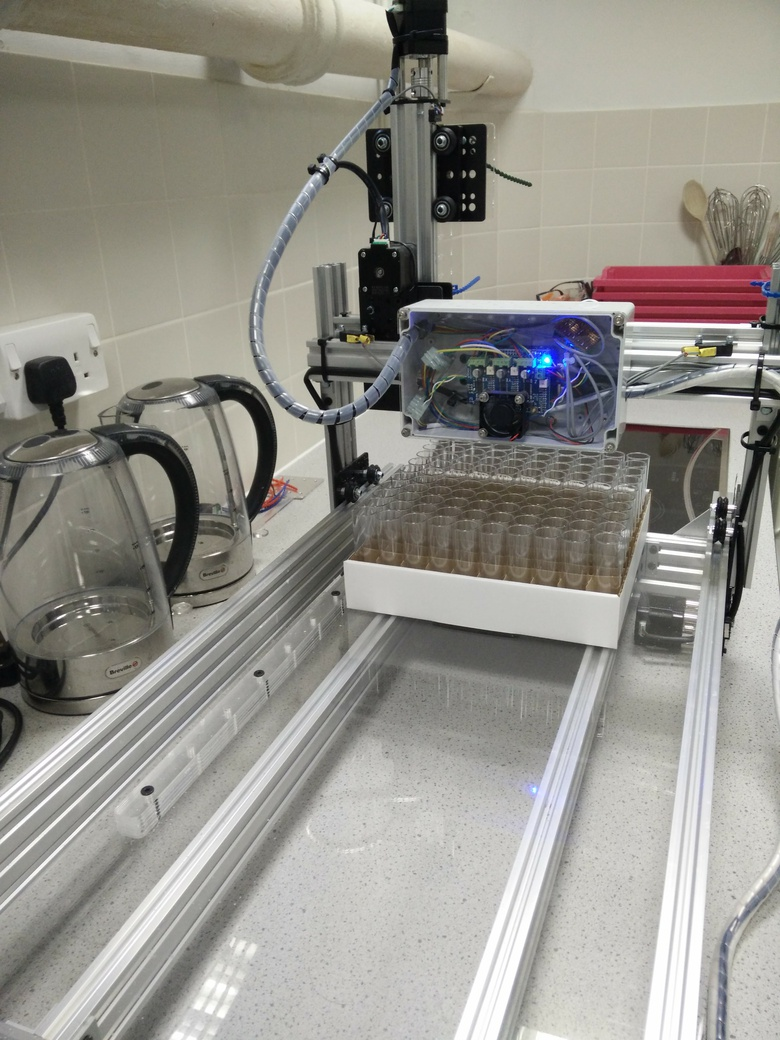
\includegraphics[width=0.5\linewidth]{images/one_box_loaded} 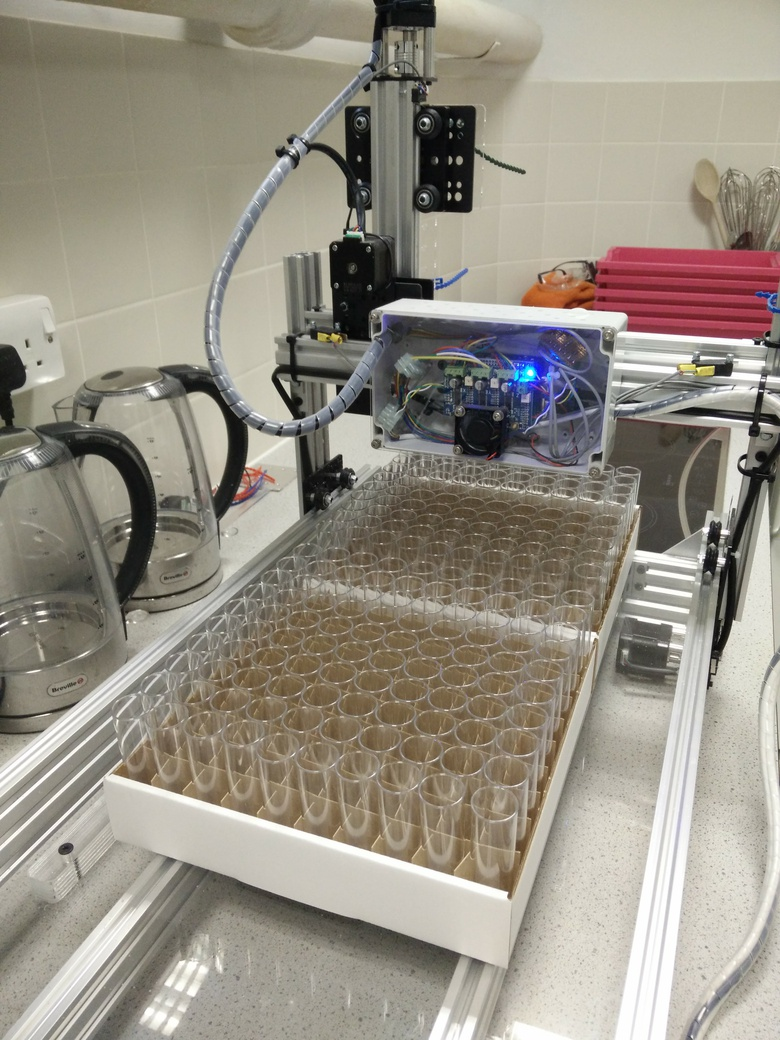
\includegraphics[width=0.5\linewidth]{images/two_boxes_loaded} 

}

\caption{Loading boxes of vials.}\label{fig:loadBoxes2}
\end{figure}

Load boxes onto the platform of the robot (figure \ref{fig:loadBoxes2}).
* The first box should be flush with the fence and the guide rail.
* The second box should be flush with the first and the guide rail.
* The boxes we are using have a pair of double-thickness side-walls and a pair of single-thickness side-walls. The pairs are on opposite sides of the box. With this type of box it is important to note the orientation of the boxes when the Cartesian coordinates of the vials are determined, because the same orientation must be used when filling vials with food. We load the boxes with a double-thickness side-wall facing forwards.

\hypertarget{boxCoordinates}{%
\section{Determine box coordinates}\label{boxCoordinates}}

We need to determine the Cartesian coordinates of vials in diagonally opposite corners of each box.

\begin{enumerate}
\def\labelenumi{\arabic{enumi}.}
\tightlist
\item
  Login to raspberry pi using ssh. My raspberry pi has the IP address 192.168.1.3 and so I would use:
\end{enumerate}

\begin{itemize}
\tightlist
\item
  \texttt{ssh\ pi@192.168.1.3}
\item
  Default password for the \textbf{pi} user account is `raspberry'.
\end{itemize}

\begin{enumerate}
\def\labelenumi{\arabic{enumi}.}
\setcounter{enumi}{1}
\tightlist
\item
  Use minicom to connect to the Grbl controller running on the Arduino, so that we can interactively control the robot from the command line:
\end{enumerate}

\begin{verbatim}
sudo minicom -D /dev/ttyACM0 -b115200
\end{verbatim}

\begin{enumerate}
\def\labelenumi{\arabic{enumi}.}
\setcounter{enumi}{2}
\tightlist
\item
  Make sure nozzle is at ** home ** position by issuing homing command:
\end{enumerate}

\begin{verbatim}
$h
\end{verbatim}

\begin{enumerate}
\def\labelenumi{\arabic{enumi}.}
\setcounter{enumi}{3}
\tightlist
\item
  First we will determine the Cartesian coordinates of the vial in the front left corner of the first box.
\end{enumerate}

\begin{itemize}
\tightlist
\item
  Make small movements in X and Y until the nozzle is centred over this vial, \emph{e.g.}:
\end{itemize}

\begin{verbatim}
x-8 y-8
\end{verbatim}

\begin{itemize}
\tightlist
\item
  Lower the nozzle in small increments until it is just 2-3mm above the the top of the vial (figure \ref{fig:box1FrontLeft}), \emph{e.g.}:
\end{itemize}

\begin{verbatim}
z-20
\end{verbatim}

\begin{itemize}
\tightlist
\item
  Query the current X, Y and Z coordinates by issuing the following command:
\end{itemize}

\begin{verbatim}
?
\end{verbatim}

Make a note of all three coordinates.

\begin{figure}

{\centering 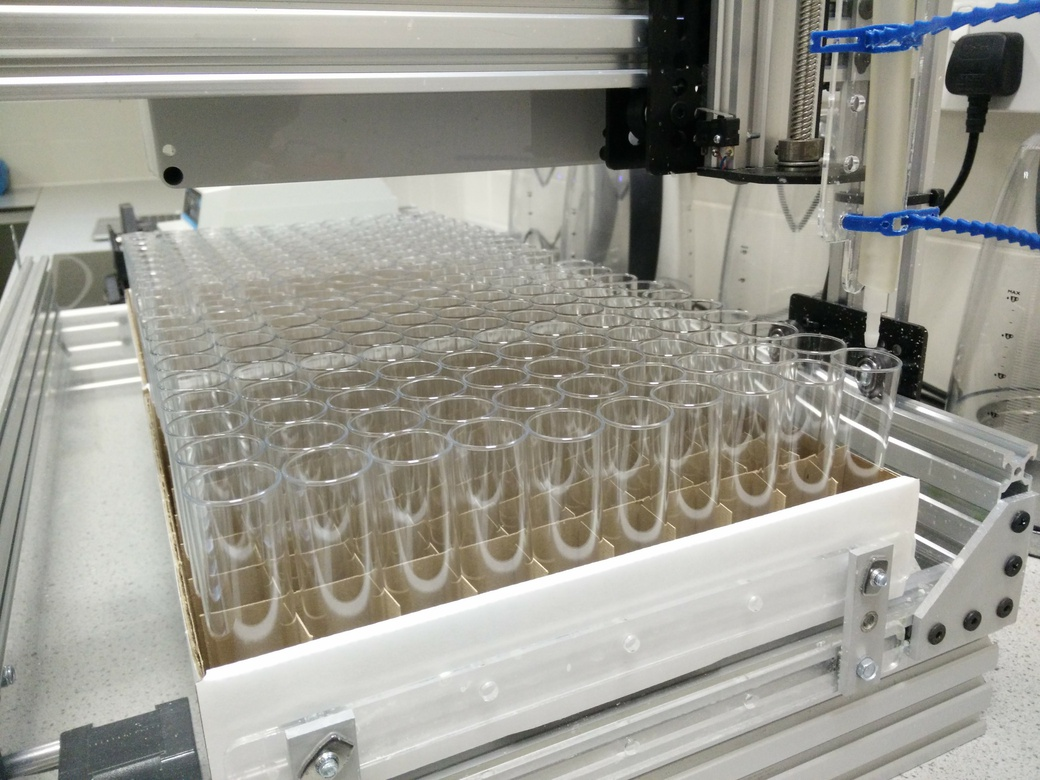
\includegraphics[width=0.5\linewidth]{images/box1_first_vial} 

}

\caption{Nozzle positioned over the front left vial in box 1.}\label{fig:box1FrontLeft}
\end{figure}

\begin{enumerate}
\def\labelenumi{\arabic{enumi}.}
\setcounter{enumi}{4}
\tightlist
\item
  Issue G-code commands to move the nozzle laterally until it is over the back right vial of the first box (figure \ref{fig:box1BackRight}).
\end{enumerate}

\begin{figure}

{\centering 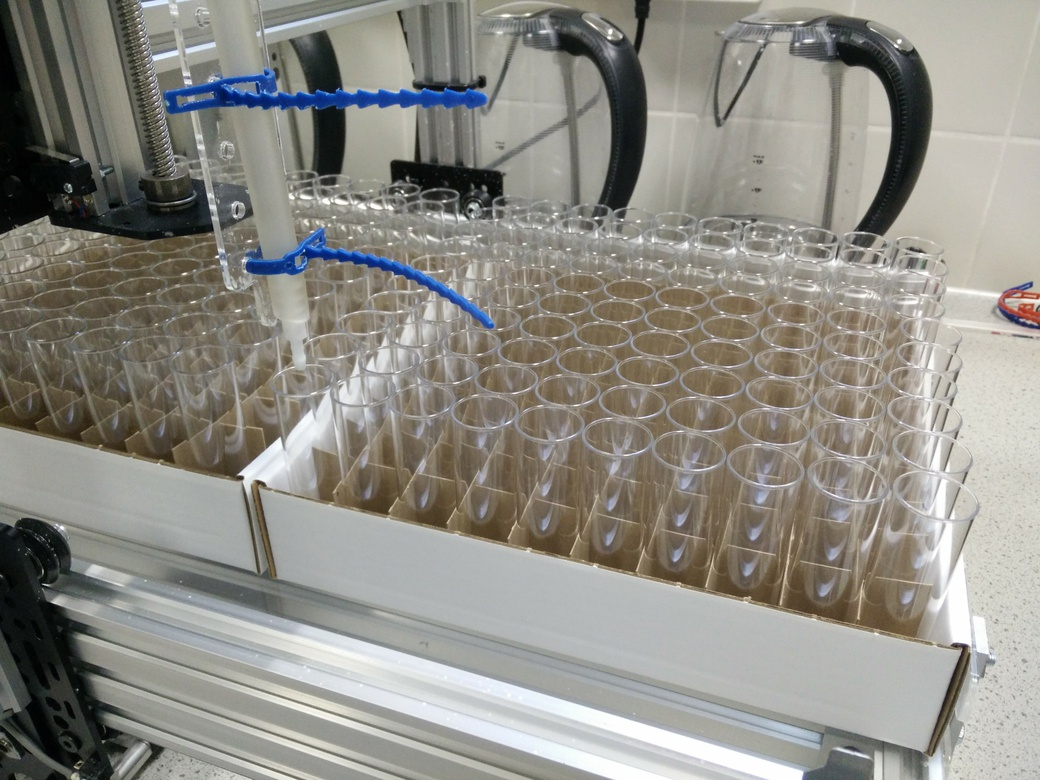
\includegraphics[width=0.5\linewidth]{images/box1_last_vial} 

}

\caption{Nozzle positioned over the back right vial in box 1.}\label{fig:box1BackRight}
\end{figure}

\begin{itemize}
\tightlist
\item
  Use \texttt{?} command to query nozzle position, and make a note of the X and Y coordinates:
\end{itemize}

\begin{enumerate}
\def\labelenumi{\arabic{enumi}.}
\setcounter{enumi}{5}
\tightlist
\item
  Move the nozzle laterally until it is over the front left vial of the second box (figure \ref{fig:box2FrontLeft}), then record X and Y coordinates.
\end{enumerate}

\begin{figure}

{\centering 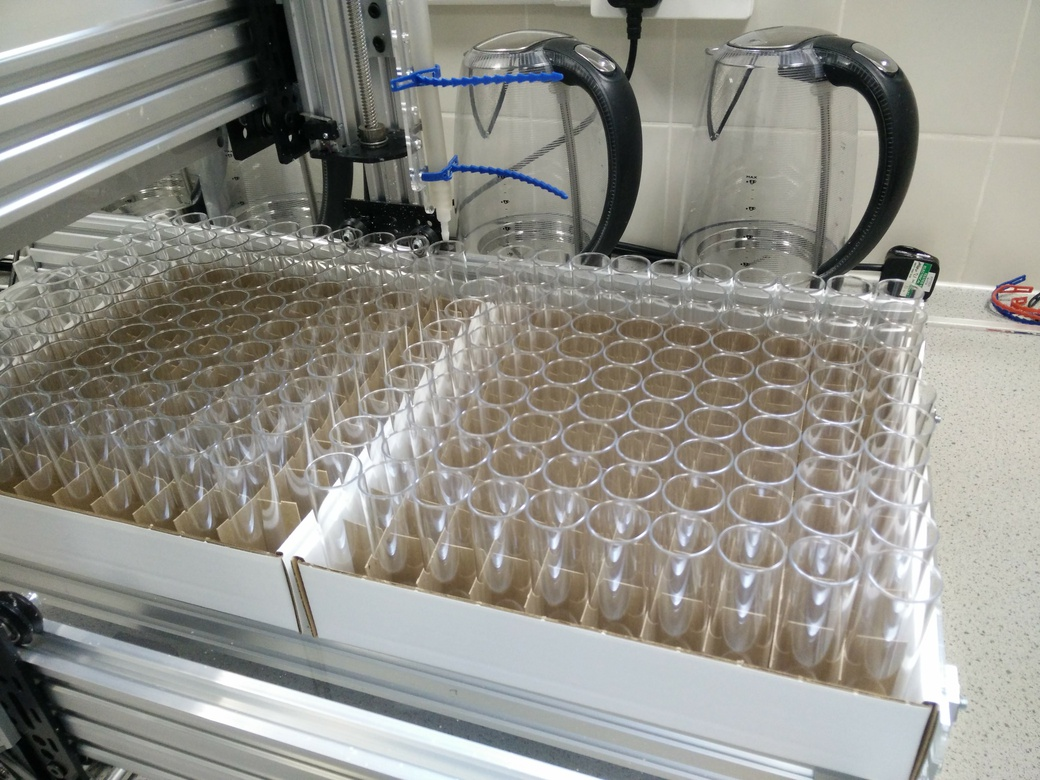
\includegraphics[width=0.5\linewidth]{images/box2_first_vial} 

}

\caption{Nozzle positioned over the front left vial in box 2.}\label{fig:box2FrontLeft}
\end{figure}

\begin{enumerate}
\def\labelenumi{\arabic{enumi}.}
\setcounter{enumi}{6}
\tightlist
\item
  Finally determine the X and Y coordinates of the back right vial in the second box (figure \ref{fig:box2BackRight}).
\end{enumerate}

\begin{figure}

{\centering 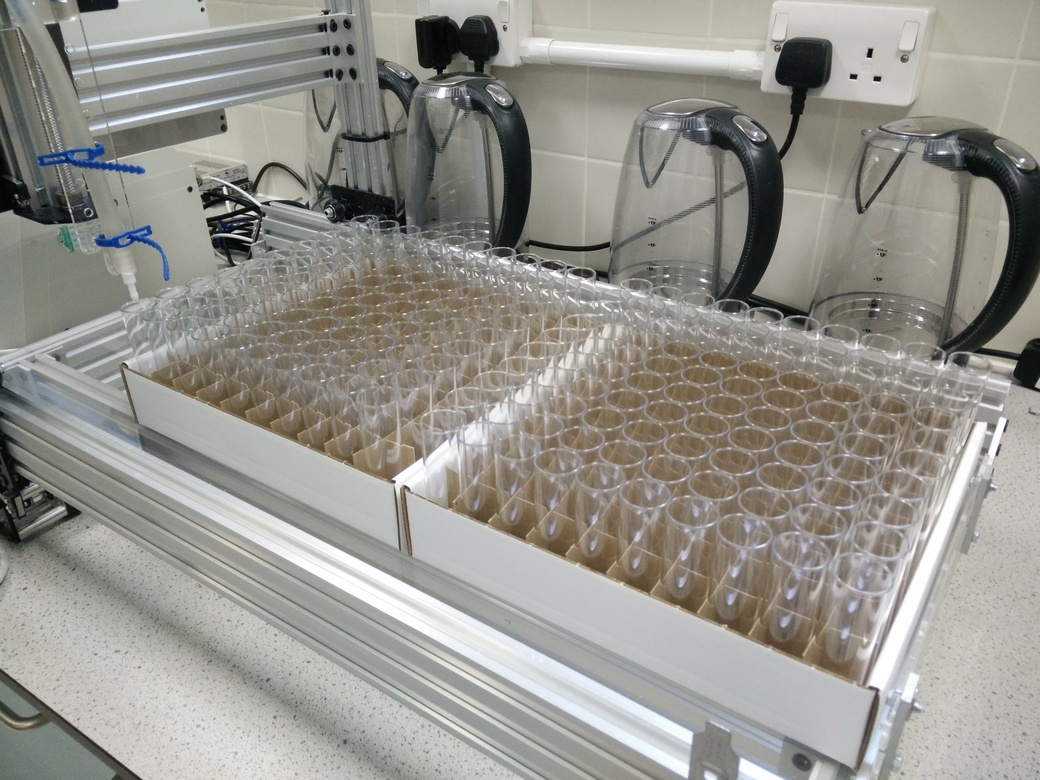
\includegraphics[width=0.5\linewidth]{images/box2_last_vial} 

}

\caption{Nozzle positioned over the back right vial in box 2.}\label{fig:box2BackRight}
\end{figure}

\hypertarget{calibratePump}{%
\section{Calibrate pump}\label{calibratePump}}

The peristaltic pump is started and stopped using the \texttt{m8} and \texttt{m9} G-code commands, respectively (table \ref{tab:gCodes}). To maximize speed, the pump will be run at its maximum flow rate of 30ml/second. In our fly facility, we add 9ml of food to each vial, therefore based on the maximum flow rate, we should only need to run the pump for 0.3 seconds to dispense 9ml of food. However, there is latency in the system and the pump does not reach its maximum flow rate instantaneously on activation. Therefore, it is important to determine the \emph{fill time} empirically. We do this by programming the robot to test fill a single box of vials using a range of \emph{fill times}. The \textbf{calibrate\_pump.py} script downloaded to the Raspberry Pi in stage \ref{installScripts} can be used to generate the appropriate G-code program.

\begin{enumerate}
\def\labelenumi{\arabic{enumi}.}
\tightlist
\item
  Open \textbf{calibrate\_pump.py} for editing:
\end{enumerate}

\begin{verbatim}
sudo nano /home/pi/robot/py/calibrate_pump.py
\end{verbatim}

\begin{enumerate}
\def\labelenumi{\arabic{enumi}.}
\setcounter{enumi}{1}
\tightlist
\item
  Near the top of the file (line 32 onwards) are various settings to be modified:
\end{enumerate}

\begin{verbatim}

# SETTINGS

# filename
filename = '/home/pi/robot/nc/calibrate_pump.nc'

# home/datum + homing pull-off (mm) (value of Grbl setting $27)
x_home = -5
y_home = -5
z_home = -5

# z value providing minimal clearance between nozzle and top of vials
z_fill = -62 

# peristaltic pump settings
min_fill_time = 0.3
max_fill_time = 0.6
# pause to allow for drips before moving to next vial
drip_pause = 0.1 

# vial coordinates (x,y)
frontLeft = (-8,-14)
backRight = (-236,-240)

nrows=10
ncols=10
\end{verbatim}

\begin{itemize}
\tightlist
\item
  The \textbf{filename} is the full path to the G-code file that will be generated by the python script.
\item
  The parameters \textbf{x\_home, y\_home} and \textbf{z\_home} are the Cartesian coordinates of the home position (\emph{i.e.} home/datum + homing pull-off (mm)).
\item
  Modify \textbf{z\_fill} to the appropriate nozzle height for filling vials (this was determined in step 5 of section \ref{boxCoordinates}).
\item
  The \textbf{min\_fill\_time} should be set to our estimate of \emph{fill time} based on the pump's specified flow rate. We will set \textbf{max\_fill\_time} to twice the value of \textbf{min\_fill\_time}.
\item
  The vial coordinates (\textbf{frontLeft} and \textbf{frontRight}) are those determined for the front left and back right vials in the first box (refer to steps 5 and 6 of section \ref{boxCoordinates}).
\item
  Our boxes have ten rows, each containing ten vials, so we set \textbf{nrows} and \textbf{ncols} to 10.
\end{itemize}

\begin{enumerate}
\def\labelenumi{\arabic{enumi}.}
\setcounter{enumi}{2}
\tightlist
\item
  After editing the settings in \textbf{calibrate\_pump.py}, run the script to generate a G-code program:
\end{enumerate}

\begin{verbatim}
./robot/py/calibrate_pump.py
\end{verbatim}

This will generate a G-code program: \textbf{/home/pi/robot/nc/calibrate\_pump.nc} which will iteratively increase the fill time for each successive row of vials. The \textbf{min\_fill\_time} will be used for the first row of vials and the fill time will be increased by (\textbf{max\_fill\_time} - \textbf{min\_fill\_time}) / (\textbf{nrows} - 1.0) for each successive row (\emph{e.g.} table \ref{tab:calibrationFillTimes}). Note that the fill times are rounded to the nearest 100th of a second. The fill time for each row is listed in the comments at the top of the \textbf{/home/pi/robot/nc/calibrate\_pump.nc} file; to view this information run:

\begin{verbatim}
head -n12 ~/robot/nc/calibrate_pump.nc
\end{verbatim}

\begin{table}

\caption{\label{tab:calibrationFillTimes}Example calibration fill times.}
\centering
\begin{tabular}[t]{rr}
\toprule
Box Row & Fill Time\\
\midrule
1 & 0.30\\
2 & 0.33\\
3 & 0.37\\
4 & 0.40\\
5 & 0.43\\
\addlinespace
6 & 0.47\\
7 & 0.50\\
8 & 0.53\\
9 & 0.57\\
10 & 0.60\\
\bottomrule
\end{tabular}
\end{table}

\begin{enumerate}
\def\labelenumi{\arabic{enumi}.}
\setcounter{enumi}{3}
\tightlist
\item
  Send the G-code pump-calibration program to the Grbl controller
  \textbf{/home/pi/robot/py/stream2.py} can be used to stream a text file of G-code commands to Grbl:
\end{enumerate}

\begin{verbatim}
./robot/py/stream2.py robot/nc/calibrate_pump.nc /dev/ttyACM0
\end{verbatim}

Once the robot has completed the calibration run and returned the nozzle to the home position, inspect the fill level in each row of vials. Identify the row in which vials are filled with the desired volume of food and then refer to the \textbf{/home/pi/robot/calibrate\_pump.nc} file to find out the fill time used for that particular row.

\hypertarget{generate-programs}{%
\section{Generate programs}\label{generate-programs}}

Once the pump has been calibrated we are ready to generate the G-code instructions for the routine filling of vials. The \textbf{fill\_boxes.py} script downloaded to the Raspberry Pi in stage \ref{installScripts} is used to generate two G-code programs:

\begin{itemize}
\tightlist
\item
  \textbf{1\_box.nc} - fill one box of vials
\item
  \textbf{2\_boxes.nc} - fill two boxes of vials
\end{itemize}

\begin{enumerate}
\def\labelenumi{\arabic{enumi}.}
\tightlist
\item
  Open \textbf{fill\_boxes.py} for editing:
\end{enumerate}

\begin{verbatim}
sudo nano /home/pi/robot/py/fill_boxes.py
\end{verbatim}

\begin{enumerate}
\def\labelenumi{\arabic{enumi}.}
\setcounter{enumi}{1}
\tightlist
\item
  Near the top of the file (line 32 onwards) are various settings to be modified:
\end{enumerate}

\begin{verbatim}

# SETTINGS
# modify values of variables in this section to match your system

# filenames
filename1Box = '/home/pi/robot/nc/1_box.nc'
filename2Boxes = '/home/pi/robot/nc/2_boxes.nc'

# home/datum + homing pull-off (mm) (value of Grbl setting $27)
x_home = -5
y_home = -5
z_home = -5

# z value providing minimal clearance between nozzle and top of vials
z_fill = -62 

# peristaltic pump settings
fill_time = 0.43
# pause to allow for drips before moving to next vial
drip_pause = 0.1 

# vial coordinates (x,y)
box1FrontLeft = (-8,-14)
box1BackRight = (-236,-240)
box2FrontLeft = (-8,-286)
box2BackRight = (-236,-513)

nrows=10
ncols=10
nVials=nrows*ncols
\end{verbatim}

\begin{itemize}
\tightlist
\item
  \textbf{filename1Box} and \textbf{filename2Boxes} specify the filename and full path to the two G-code programs that will be generated. You should not need to modify these values. The GUI script (\textbf{/home/pi/robot/py/fly\_gui.py}) expects the two programs to have the default names and paths; if you alter the names or paths of these files, you will need to edit the GUI script.
\item
  The parameters \textbf{x\_home, y\_home} and \textbf{z\_home} are the Cartesian coordinates of the home position (\emph{i.e.} home/datum + homing pull-off (mm)).
\item
  Modify \textbf{z\_fill} to the appropriate nozzle height for filling vials (this was determined in step 5 of section \ref{boxCoordinates}).
\item
  \textbf{fill\_time} was determined in the previous section \ref{calibratePump}.
\item
  The default value of \textbf{drip\_pause} should be appropriate for most systems.
\item
  The vial coordinates (\textbf{box1FrontLeft}, \textbf{box1BackRight}, \textbf{box2FrontLeft} and \textbf{box2BackRight}) were determined in section \ref{boxCoordinates}.
\item
  Our boxes have ten rows, each containing ten vials, so we set \textbf{nrows} and \textbf{ncols} to 10.
\end{itemize}

\begin{enumerate}
\def\labelenumi{\arabic{enumi}.}
\setcounter{enumi}{2}
\tightlist
\item
  After editing the settings in \textbf{fill\_boxes.py}, run the script to generate the two G-code programs:
\end{enumerate}

\begin{verbatim}
./robot/py/fill_boxes.py
\end{verbatim}

\hypertarget{operation}{%
\chapter{Routine operation}\label{operation}}

\hypertarget{prepare-system}{%
\section{Prepare system}\label{prepare-system}}

Instructions for starting the system are provided in chapter \ref{startup}.

\hypertarget{fill-boxes}{%
\section{Fill boxes}\label{fill-boxes}}

Load boxes onto platform as described in section \ref{loadBoxes}.

From the touchscreen menu select \textbf{1 Box} or \textbf{2 Boxes} depending on the number of boxes on the platform (figure \ref{fig:touchscreen}). The robot will \textbf{home} to zero the cartesian coordinate system, and then commence filling the vials.

\begin{figure}

{\centering 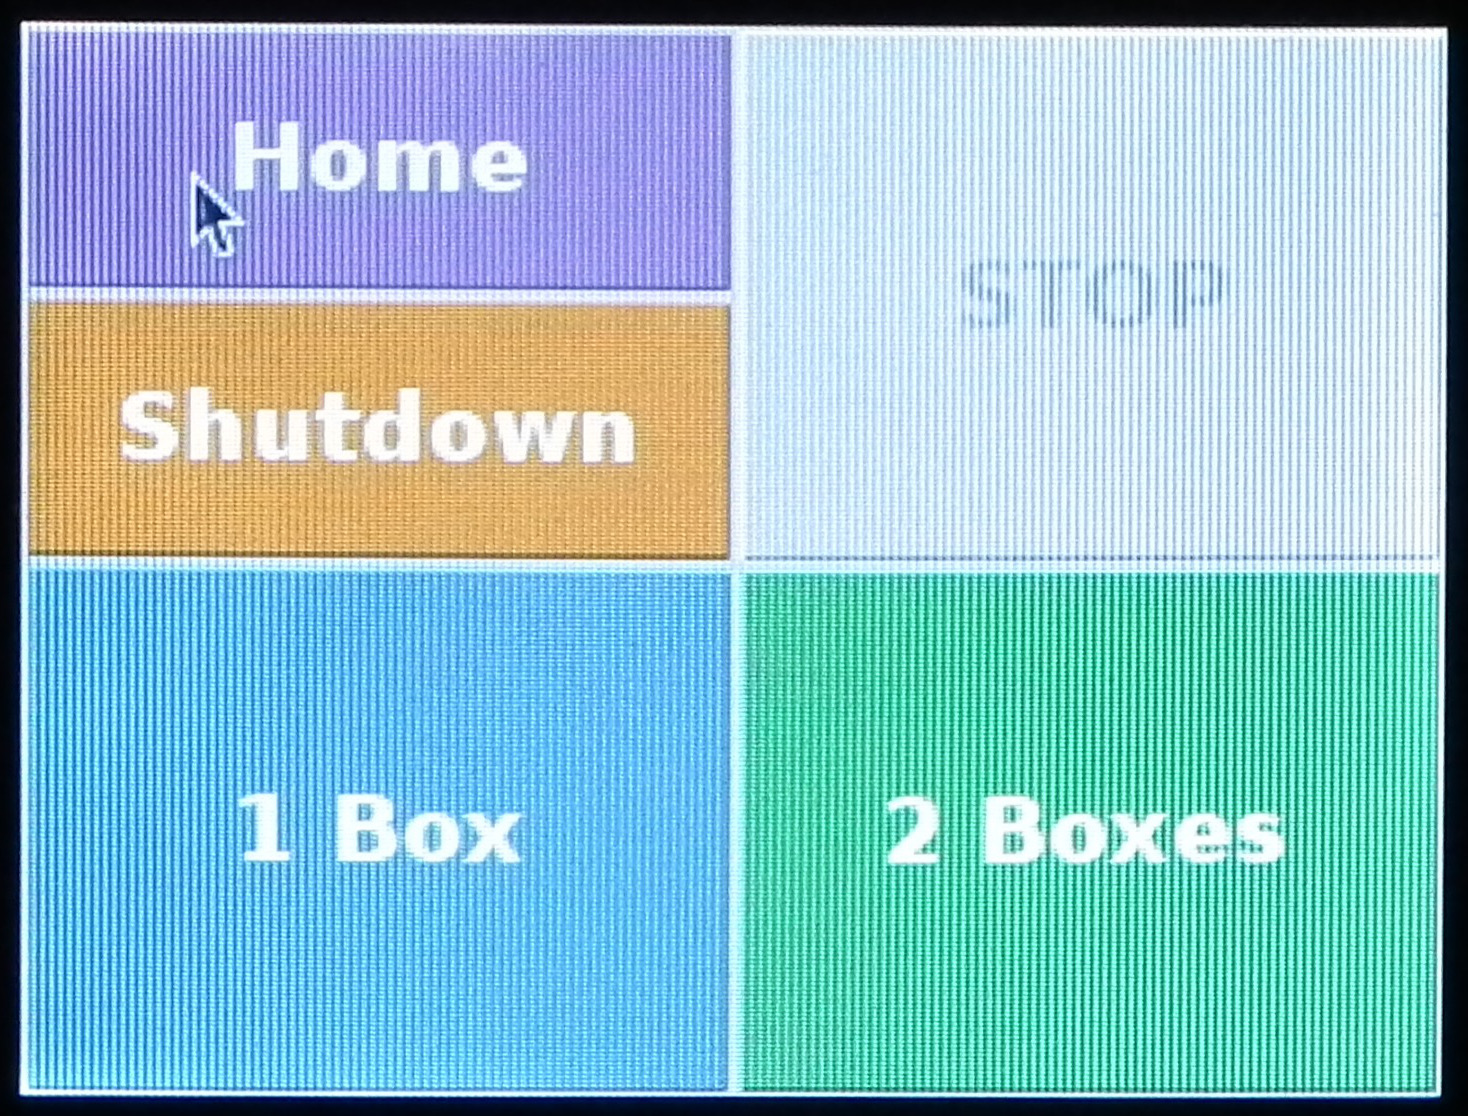
\includegraphics[width=0.6\linewidth]{images/gui} 

}

\caption{Touchscreen interface.}\label{fig:touchscreen}
\end{figure}

During filling the robot can be stopped by clicking on the \textbf{Stop} button (figure \ref{fig:stopRobot}).

\begin{figure}

{\centering 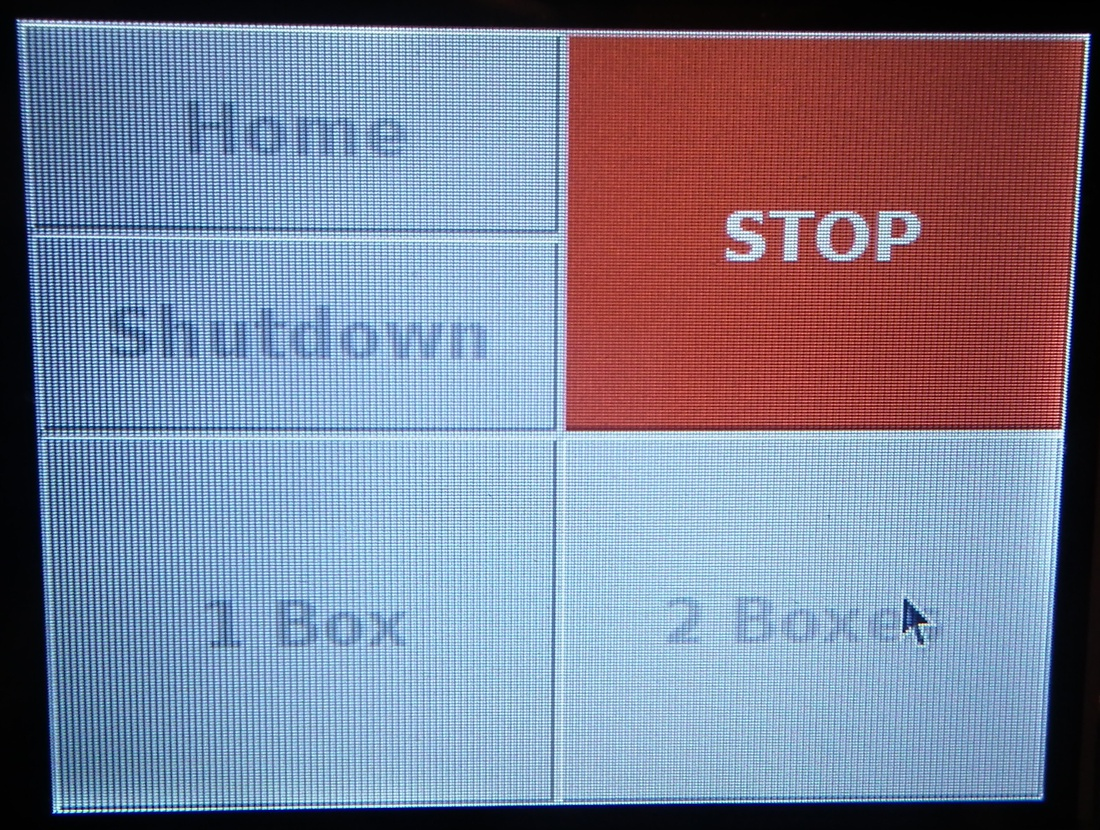
\includegraphics[width=0.6\linewidth]{images/gui_stop2} 

}

\caption{Appearance of touchscreen interface when a job is running.}\label{fig:stopRobot}
\end{figure}

\hypertarget{shutdown}{%
\section{Shutdown}\label{shutdown}}

\begin{itemize}
\tightlist
\item
  The raspberry pi should be shutdown using the \textbf{shutdown} button on the touchscreen.
\item
  The Norprene tubing should be removed from the vat of fly food, then any food remaining in the tubing can be expelled by pressing and holding the \textbf{prime} button on the peristaltic pump. Ensure there is a receptacle under the nozzle to catch the expelled fly food. The Norprene tubing should be removed from the robot for cleaning/sterilization.
\item
  All devices (raspberry pi, power supply unit for gShield and motors, and peristaltic pump) should be switched off.
\item
  The robot can be wiped clean if necessary using a damp cloth. The platform can be removed for thorough cleaning.
\end{itemize}

  \bibliography{book.bib,packages.bib}

\end{document}
